\section{Chemical and Physical Characterization of Precursors}
\label{sec:chemical_and_physical_characterization_of_precursors}

\subsection{Chemical Composition of Precursors}
\label{sec:chemical_composition_of_precursors}

The chemical composition of the aluminosilicate precursors plays a fundamental role in determining their reactivity and suitability for activation in a low-calcium system. 
In this work, the metakaolin (MK) and silica fume (SF) precursors were analysed with XRF for their oxide content (normalized with respect to the powder fraction) and loss on ignition (LOI), which was found to be 0.69\% and 2.27\%, respectively.

\begin{table}[H]
    \centering
    \caption{Chemical composition (wt \%) of the precursors: metakaolin (MK) and silica fume (SF).}
    \label{tab:xrf_mk_sf}
    \begin{tabular}{l c c c c}
        \hline
        \multirow{2}{*}{Oxide} & \multicolumn{2}{c}{Metakaolin} & \multicolumn{2}{c}{Silica Fume} \\
        \cline{2-5}
        & wt (\%) & wt with LOI (\%) & wt (\%) & wt with LOI (\%) \\
        \hline
        K\textsubscript{2}O & 0.21 & 0.20 & 0.74 & 0.73 \\
        CaO & 0.19  & 0.19 & 0.13 & 0.13 \\
        MgO & 2.60 & 2.59 & 0.00 & 0.00 \\
        Cl & 0.00 & 0.00 & 0.12 & 0.12 \\
        SO\textsubscript{3} & 0.00 & 0.00 & 0.15 & 0.15 \\
        SiO\textsubscript{2} & 49.37 & 49.03 & 96.90 & 94.70 \\
        Fe\textsubscript{2}O\textsubscript{3} & 0.77 & 0.76 & 1.78 & 1.74 \\
        Al\textsubscript{2}O\textsubscript{3} & 46.38 & 46.06 & 0.00 & 0.00 \\
        Na\textsubscript{2}O & 0.00 & 0.00 & 0.17 & 0.17 \\
        TiO\textsubscript{2} & 0.49 & 0.48 & 0.00 & 0.00 \\
        LOI &  & 0.69 &  & 2.27 \\
        \hline
    \end{tabular}
\end{table}

From Table 4.1.1 it is clear that the MK precursor is rich in alumina and contains a significant silica fraction , while the SF is extremely high in silica and essentially alumina-free.
Critically, both materials present very low CaO contents.
The minimal presence of calcium oxide is an important indicator of the low-calcium nature of the precursors, which is a pre-requisite for favoring the formation of potassium aluminosilicate hydrate type gels, rather than calcium-rich gels, as often observed when using ground granulated blast furnace slag \cite{ali2023geopolymer}.


In addition, the low LOI values suggest a limited amount of residual organics or volatile components, which could otherwise interfere with the dissolution kinetics of the aluminosilicates.
Furthermore, the Si/Al molar ratio of MK precursos is approximately 0.9, which will be used with the essentially pure SF to tailor the mix designs for optimal geopolymerization reactions, as presented in Appendix \ref{appendix:mix_designs}.

% Create a slide with this phrase:
In summary, the chemical data confirm that both MK and SF meet the key requirements of (i) high silica and/or alumina content, (ii) low calcium content, and (iii) minimal impurities, thereby validating their use as raw materials for a low calcium alkali-activated binder system.

\subsection{X-Ray Diffraction of Precursors and Alkaline Sources}
\label{sec:x-ray_diffraction_of_precursors_and_alkaline_sources}

XRD analysis of the alkaline sources revealed distinct crystalline characteristics.
The diffractogram of Ca(OH)\textsubscript{2} showed well-defined peaks corresponding to the portlandite phase (COD 900-0114), confirming its high crystallinity and purity.
Similarly, the spectrum of K\textsubscript{2}CO\textsubscript{3} exhibited reflections attributed to crystalline potassium carbonate (COD 900-9644).

These results are consistent with findings from previous studies that identified portlandite and alkali carbonates as highly crystalline solids used in geopolymer and alkali-activated systems due to their strong reactivity and predictable phase behavior \cite{Provis2014}.

The XRD patterns of SF and MK displayed broad amorphous humps, characteristic of disordered aluminosilicate and silica networks \cite{provis2009geopolymers,ke2021one}.
In MK, a diffuse hump centered around $2\theta \approx 21\degree$ was observed, with minor peaks corresponding to residual quartz (COD 900-9667), indicating the presence of impurities, which remains inert during calcination \cite{provis2014geopolymers} and acts as filler without participating in geopolymerization reaction \cite{rakhimova2019metakaolin}.
The SF diffractogram showed a similar amorphous feature near $2\theta \approx 22.5\degree$, confirming the predominance of a non-crystalline silica phase with no detectable crystalline impurities.

These findings align with the literature, where metakaolin typically exhibits a predominantly amorphous structure with residual quartz peaks depending on the calcination temperature and source clay, while silica fume is almost entirely amorphous as it is a by-product of the smelting process in silicon and ferrosilicon alloy production \cite{pachecotorgal2014handbook}.
The high amorphous content of these precursors is advantageous for geopolymerization, as it enhances the dissolution of reactive aluminosilicate species and promotes the formation of N-A-S-H and C-A-S-H type gels, leading to improved mechanical performance \cite{qin2022onepart}.

\begin{figure}[H]
    \centering
    \subfloat[Calcium Hydroxide (Ca(OH)\textsubscript{2})]{
        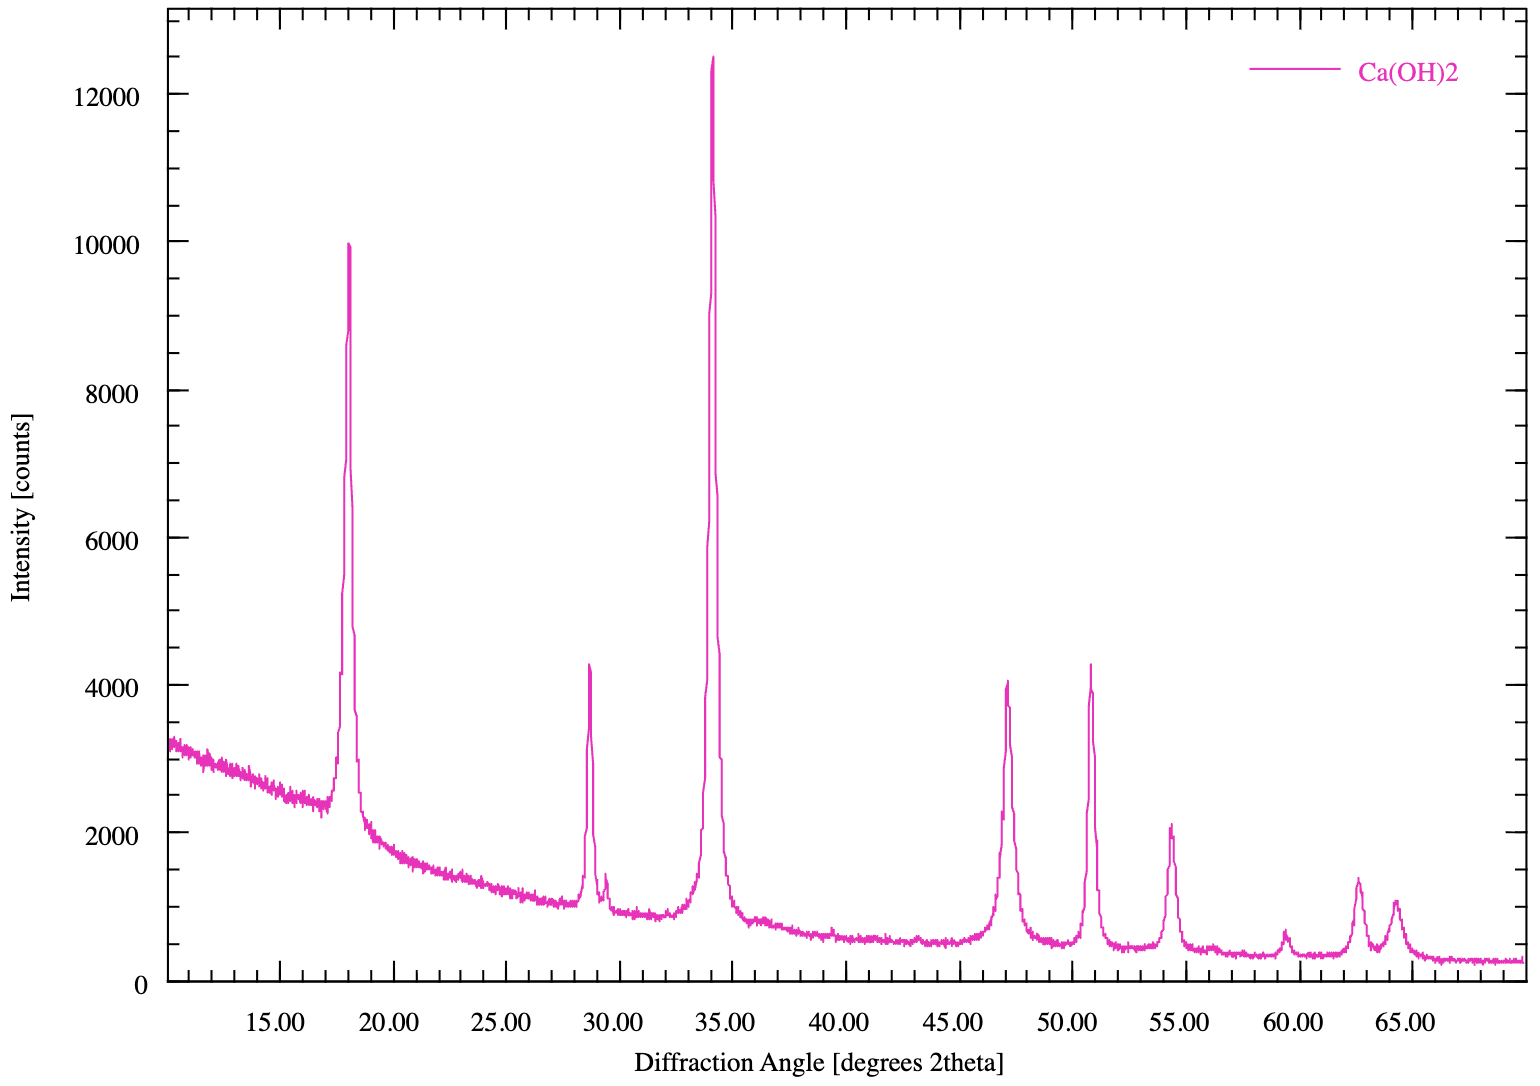
\includegraphics[width=0.45\textwidth]{Cap4/images/xrd_CH.png}
    }
    \subfloat[Potassium Carbonate (K\textsubscript{2}CO\textsubscript{3})]{
        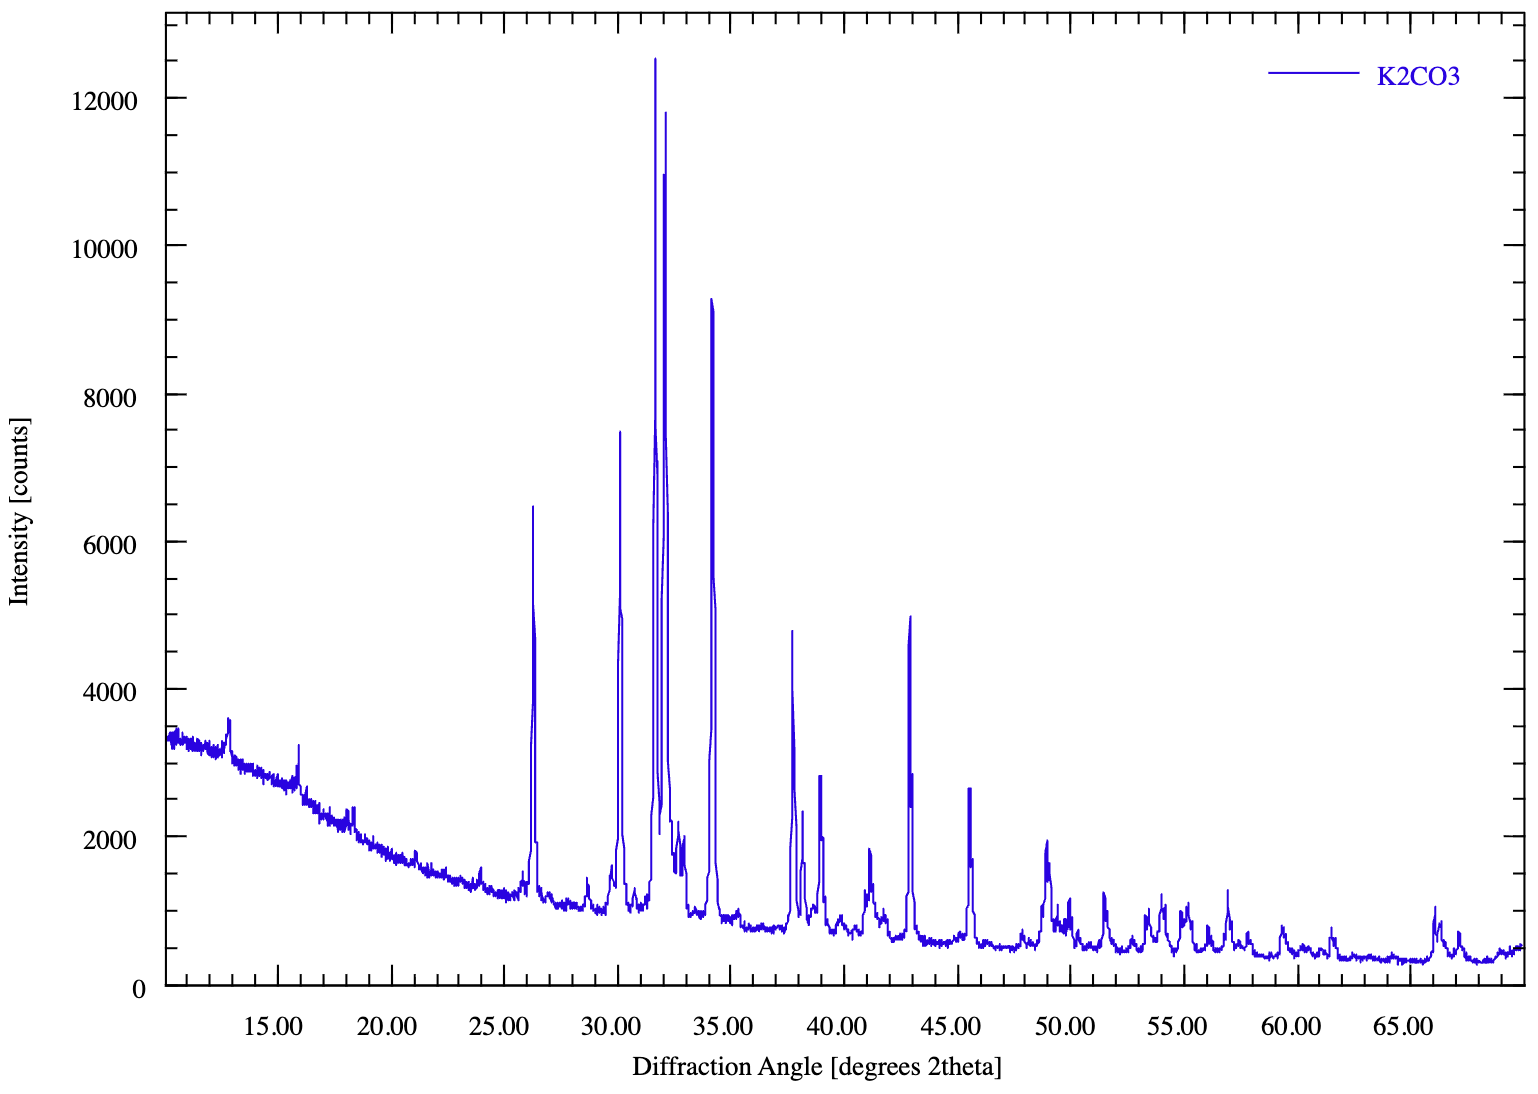
\includegraphics[width=0.45\textwidth]{Cap4/images/xrd_KC.png}
    } \\
    \subfloat[Metakaolin (MK)]{
        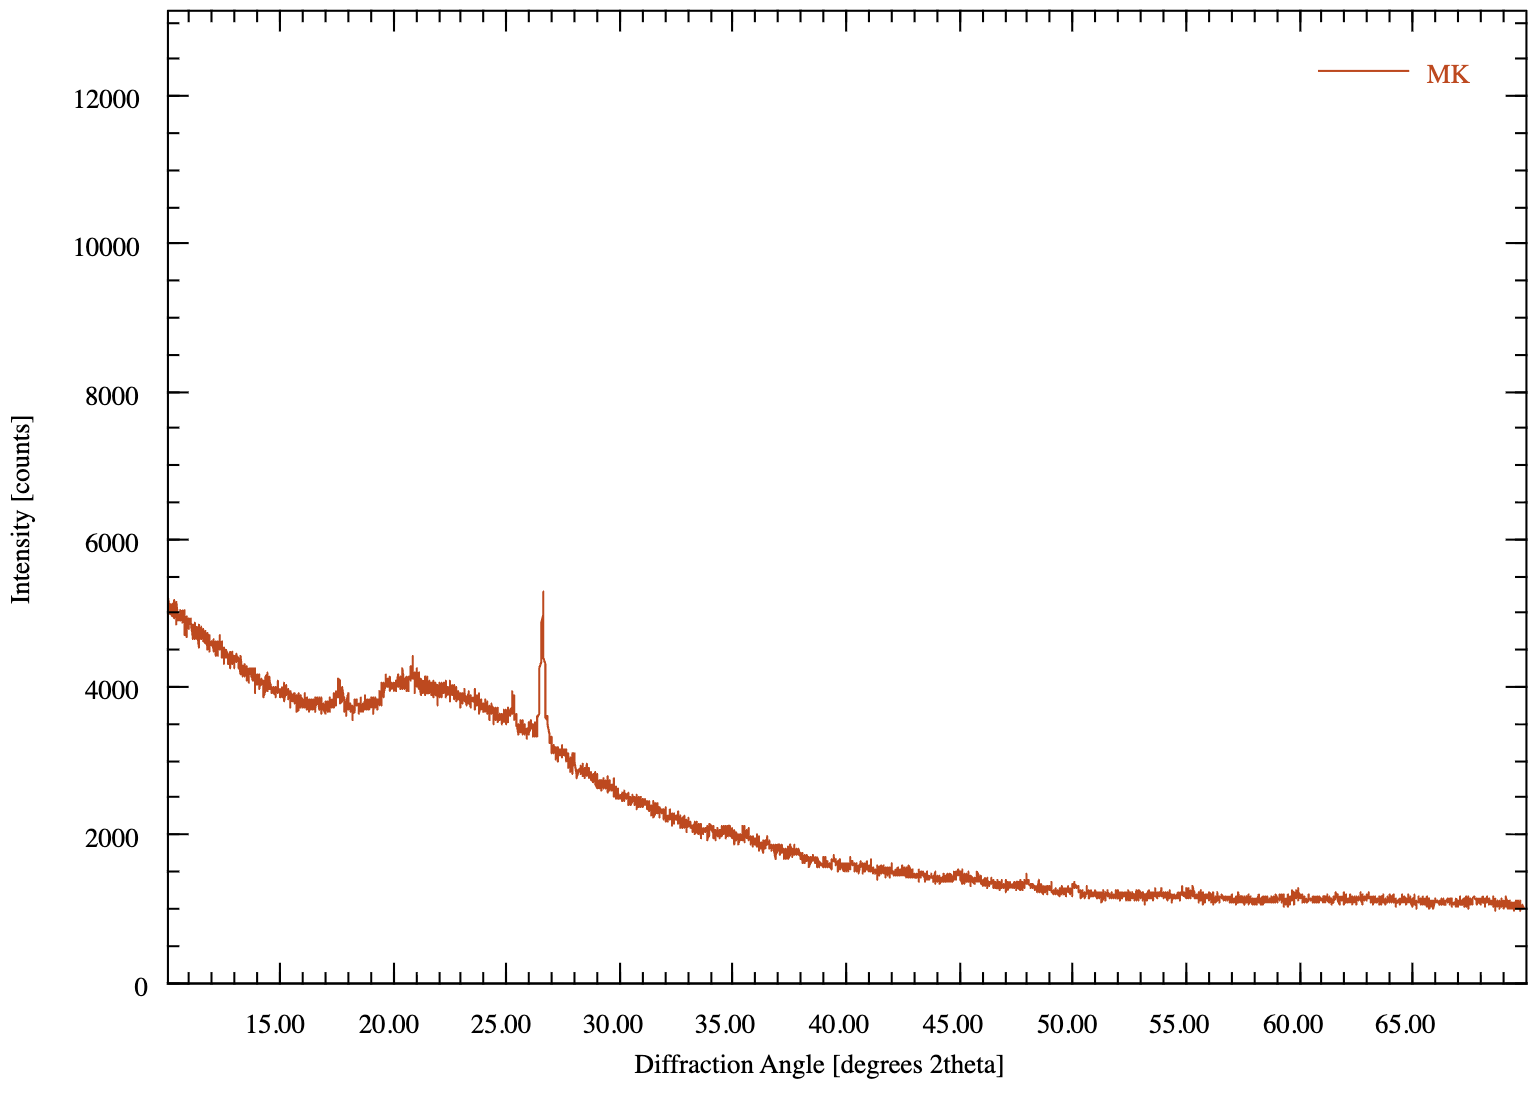
\includegraphics[width=0.45\textwidth]{Cap4/images/xrd_MK.png}
    }
    \subfloat[Silica Fume (SF)]{
        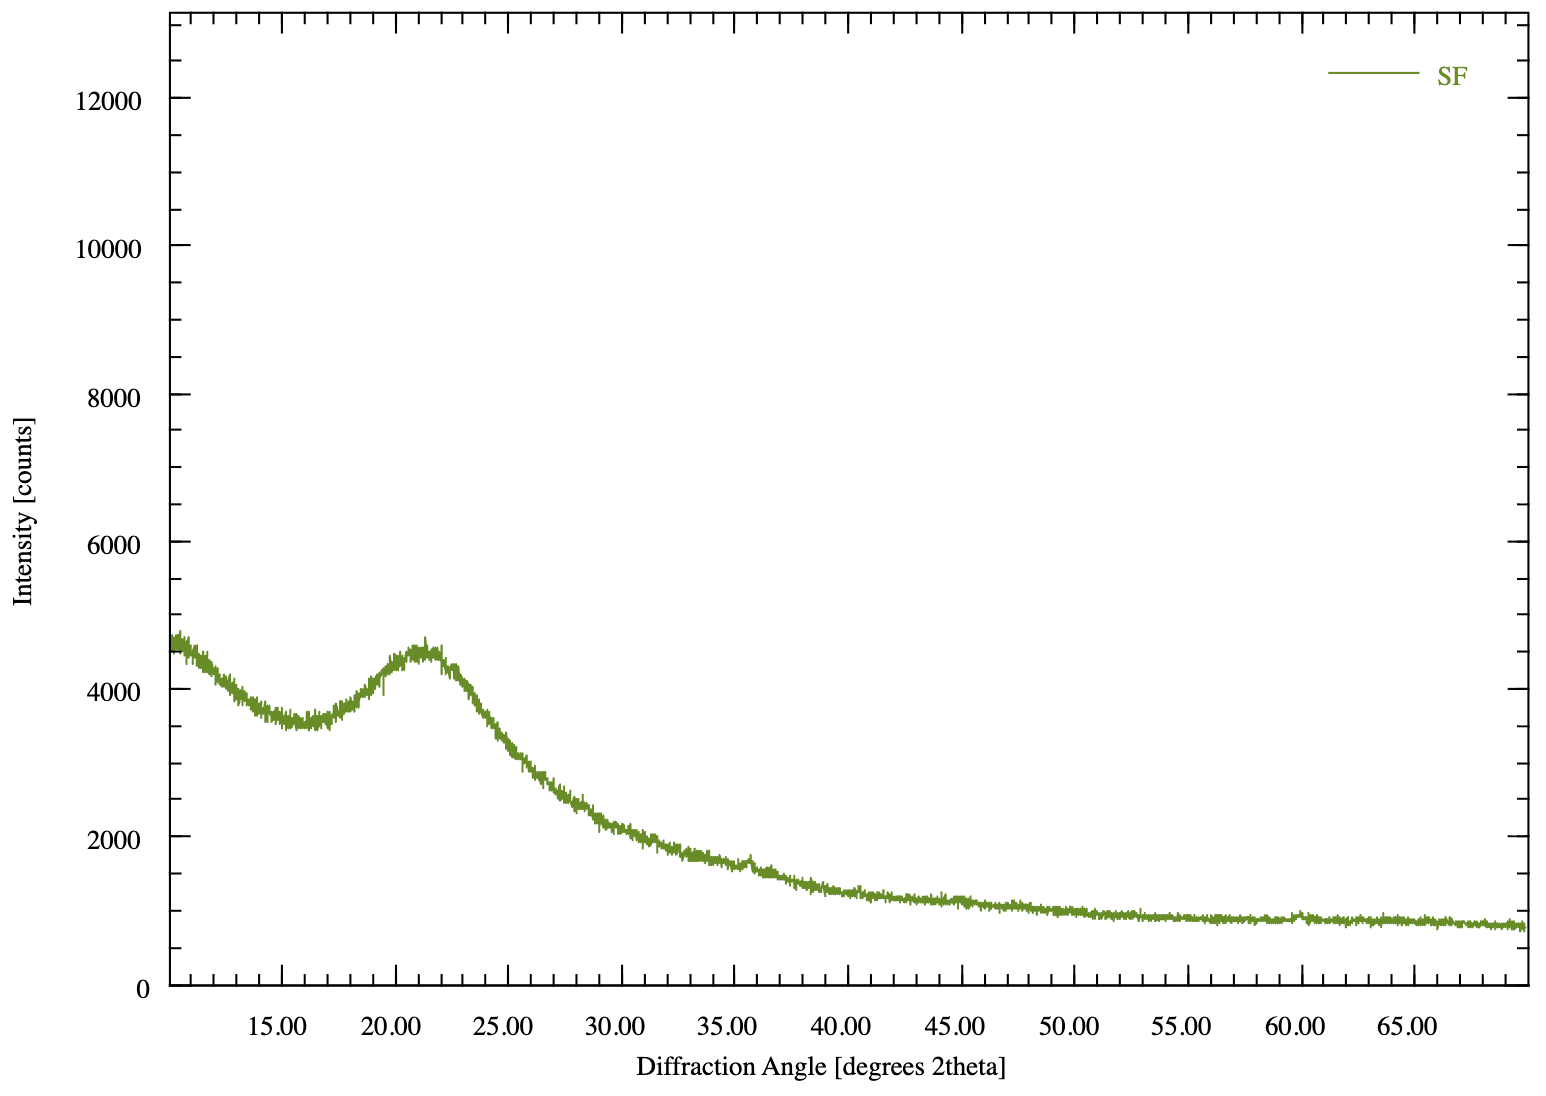
\includegraphics[width=0.45\textwidth]{Cap4/images/xrd_SF.png}
    }
    \caption{XRD patterns of solid precursors.}
    \label{fig:xrd_precursors}
\end{figure}

\subsection{Fourier Transform Infrared Spectroscopy of Precursors}

For the aluminosilicate precursors, the metakaolin exhibited three main bands at 623, 787, and 1051 cm\textsuperscript{-1}, while the silica fume showed two bands at 799 and 1040 cm\textsuperscript{-1}.
For MK, the intense band at 1051 cm\textsuperscript{-1} corresponds to the asymmetric stretching vibration of the Si-O-T bonds (where T is Si or Al) and is characteristic of its disordered aluminosilicate network, while lower wavenumber bands, such as 623 cm\textsuperscript{-1} and 787 cm\textsuperscript{-1}, relate to bending vibrations like Si-O-Al and Al-O-T \cite{moraes2024scsa}.

Conversely, the SF spectrum shows its main band at 1040cm\textsuperscript{-1}, also attributed to Si-O-T stretching, but the SF is highly pure, lacking significant Al content (as seen by the XRF results in Table \ref{tab:xrf_mk_sf}), meaning this peak is dominated by Si-O-Si bonds.
The second, smaller band near 799 cm\textsuperscript{-1} is related to the symmetric stretching of the Si-O-Si network, likely residual quartz or the amorphous silica structure \cite{ma2022calcium}.

\begin{figure}[H]
    \centering
    \subfloat[Metakaolin (MK)]{
        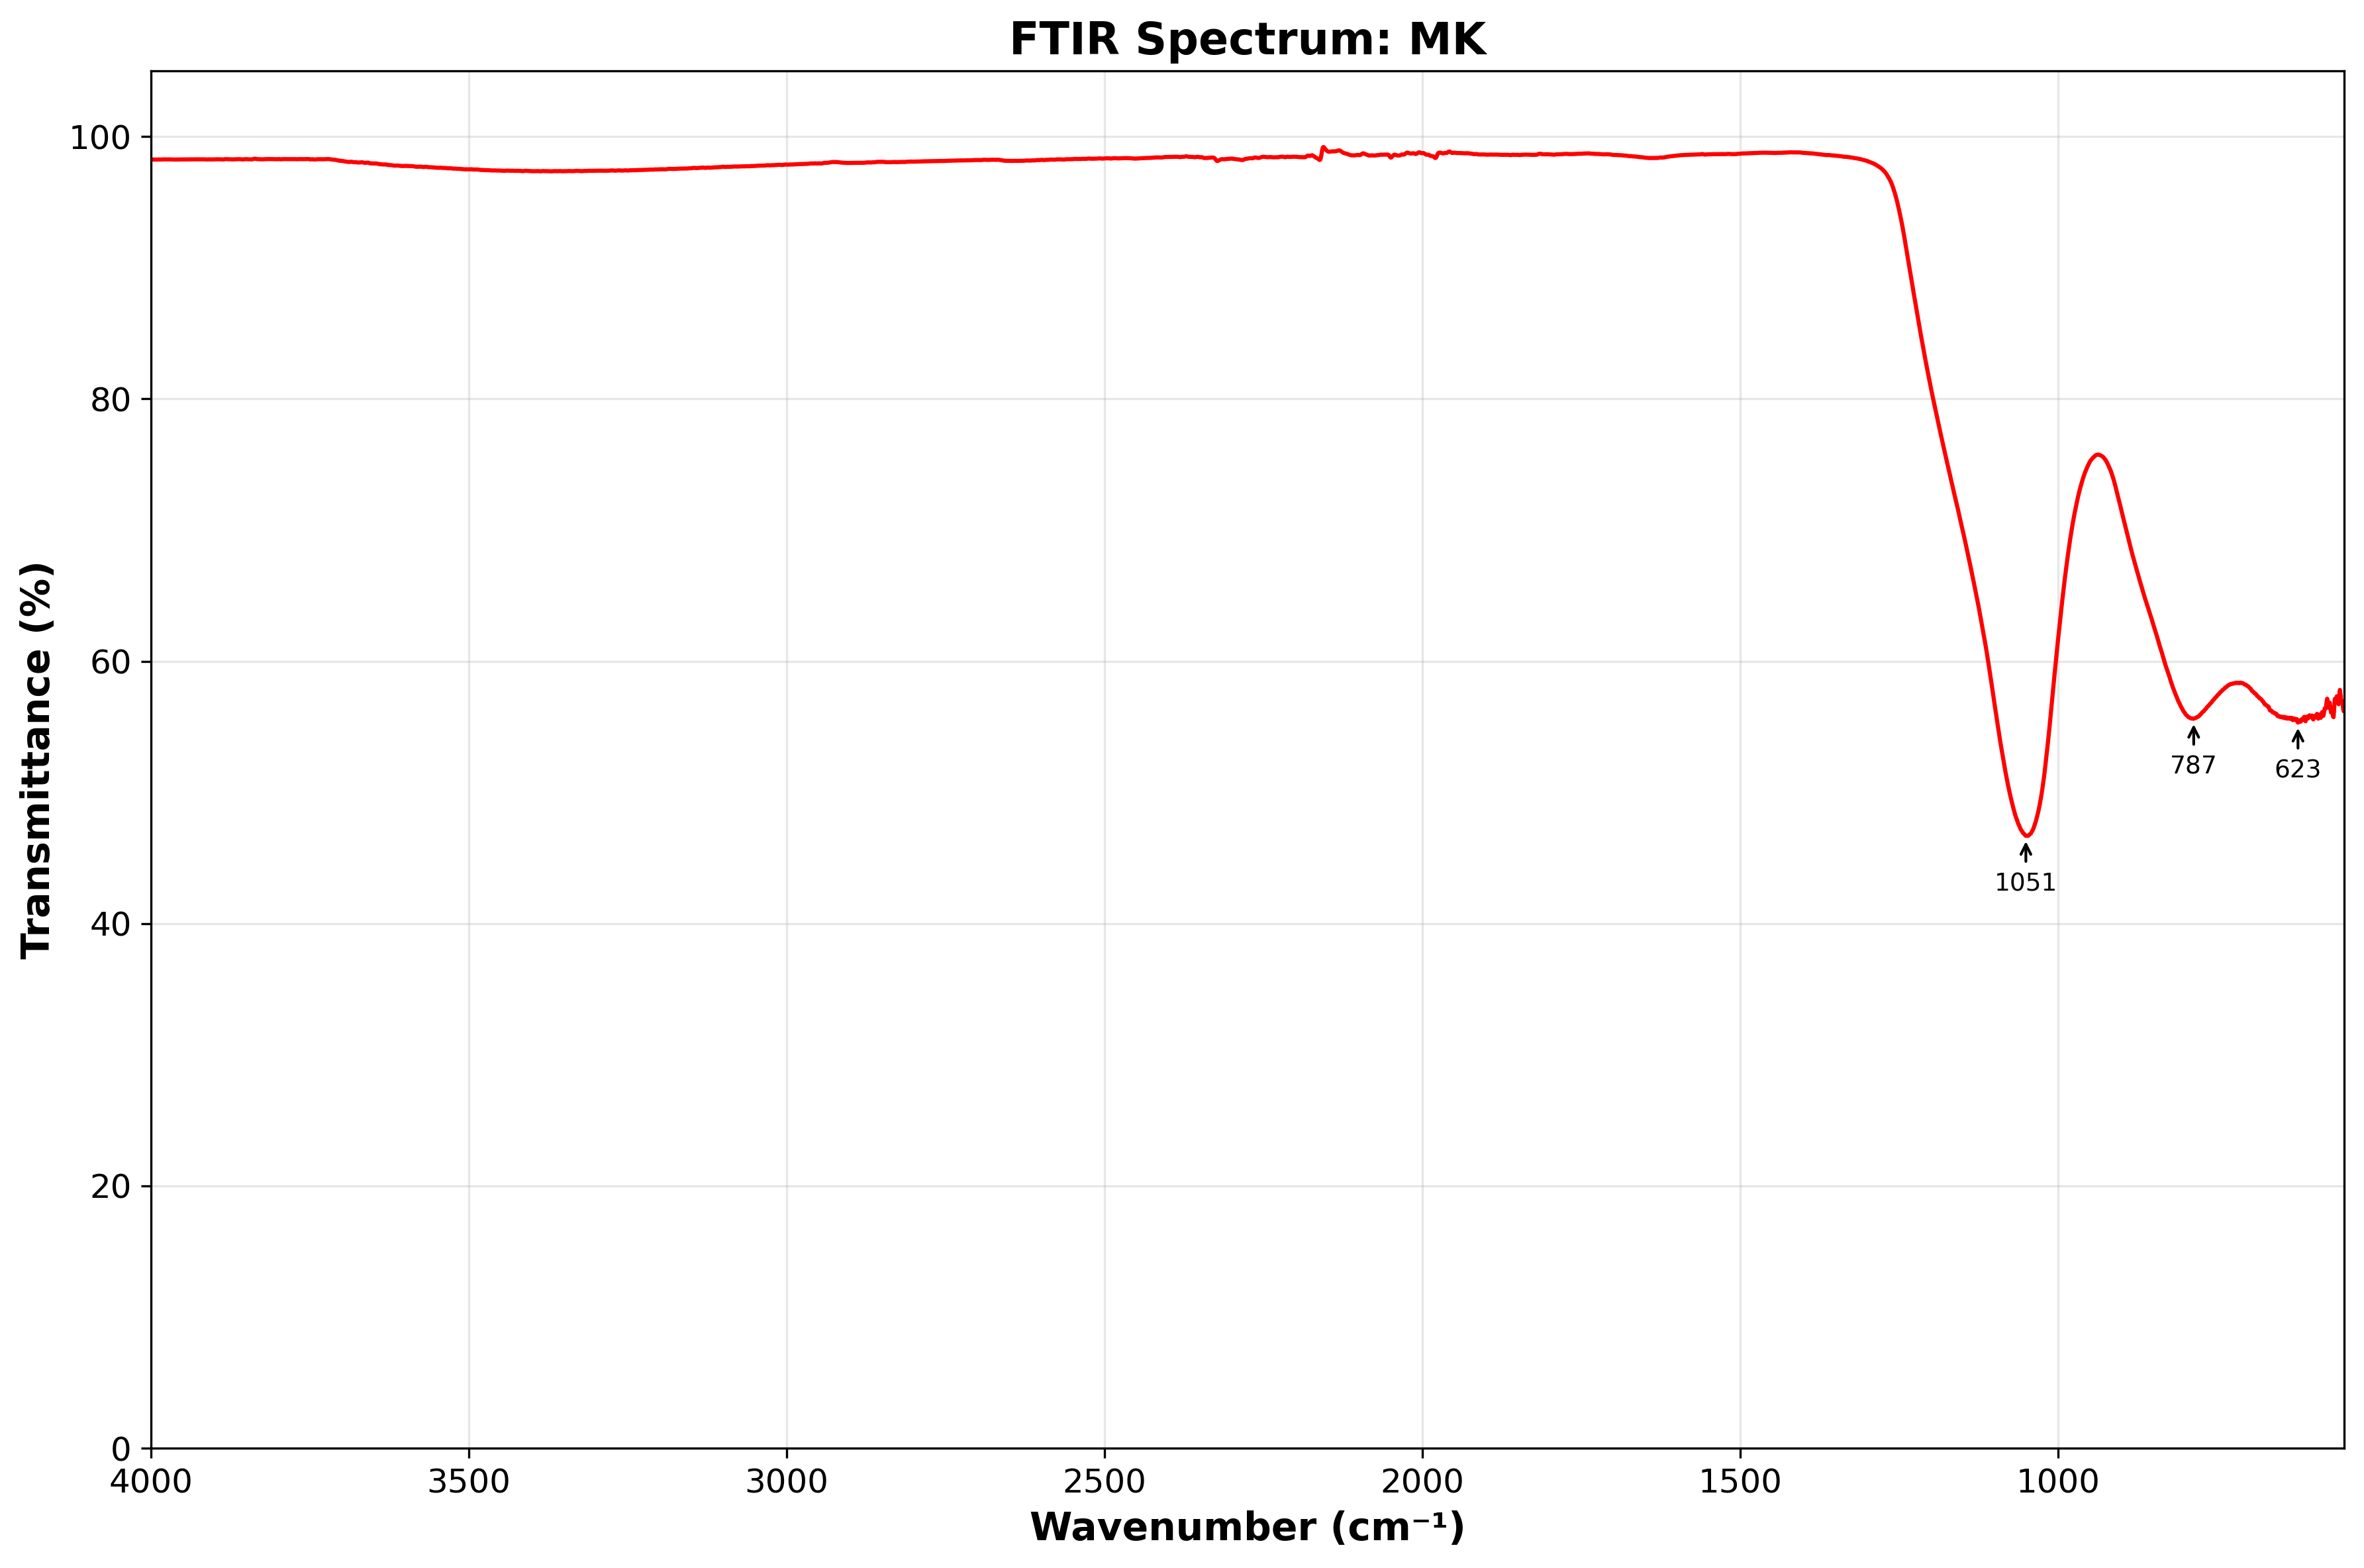
\includegraphics[width=0.475\textwidth]{Cap4/images/MK_ftir_spectrum.png}
    }
    \subfloat[Silica Fume (SF)]{
        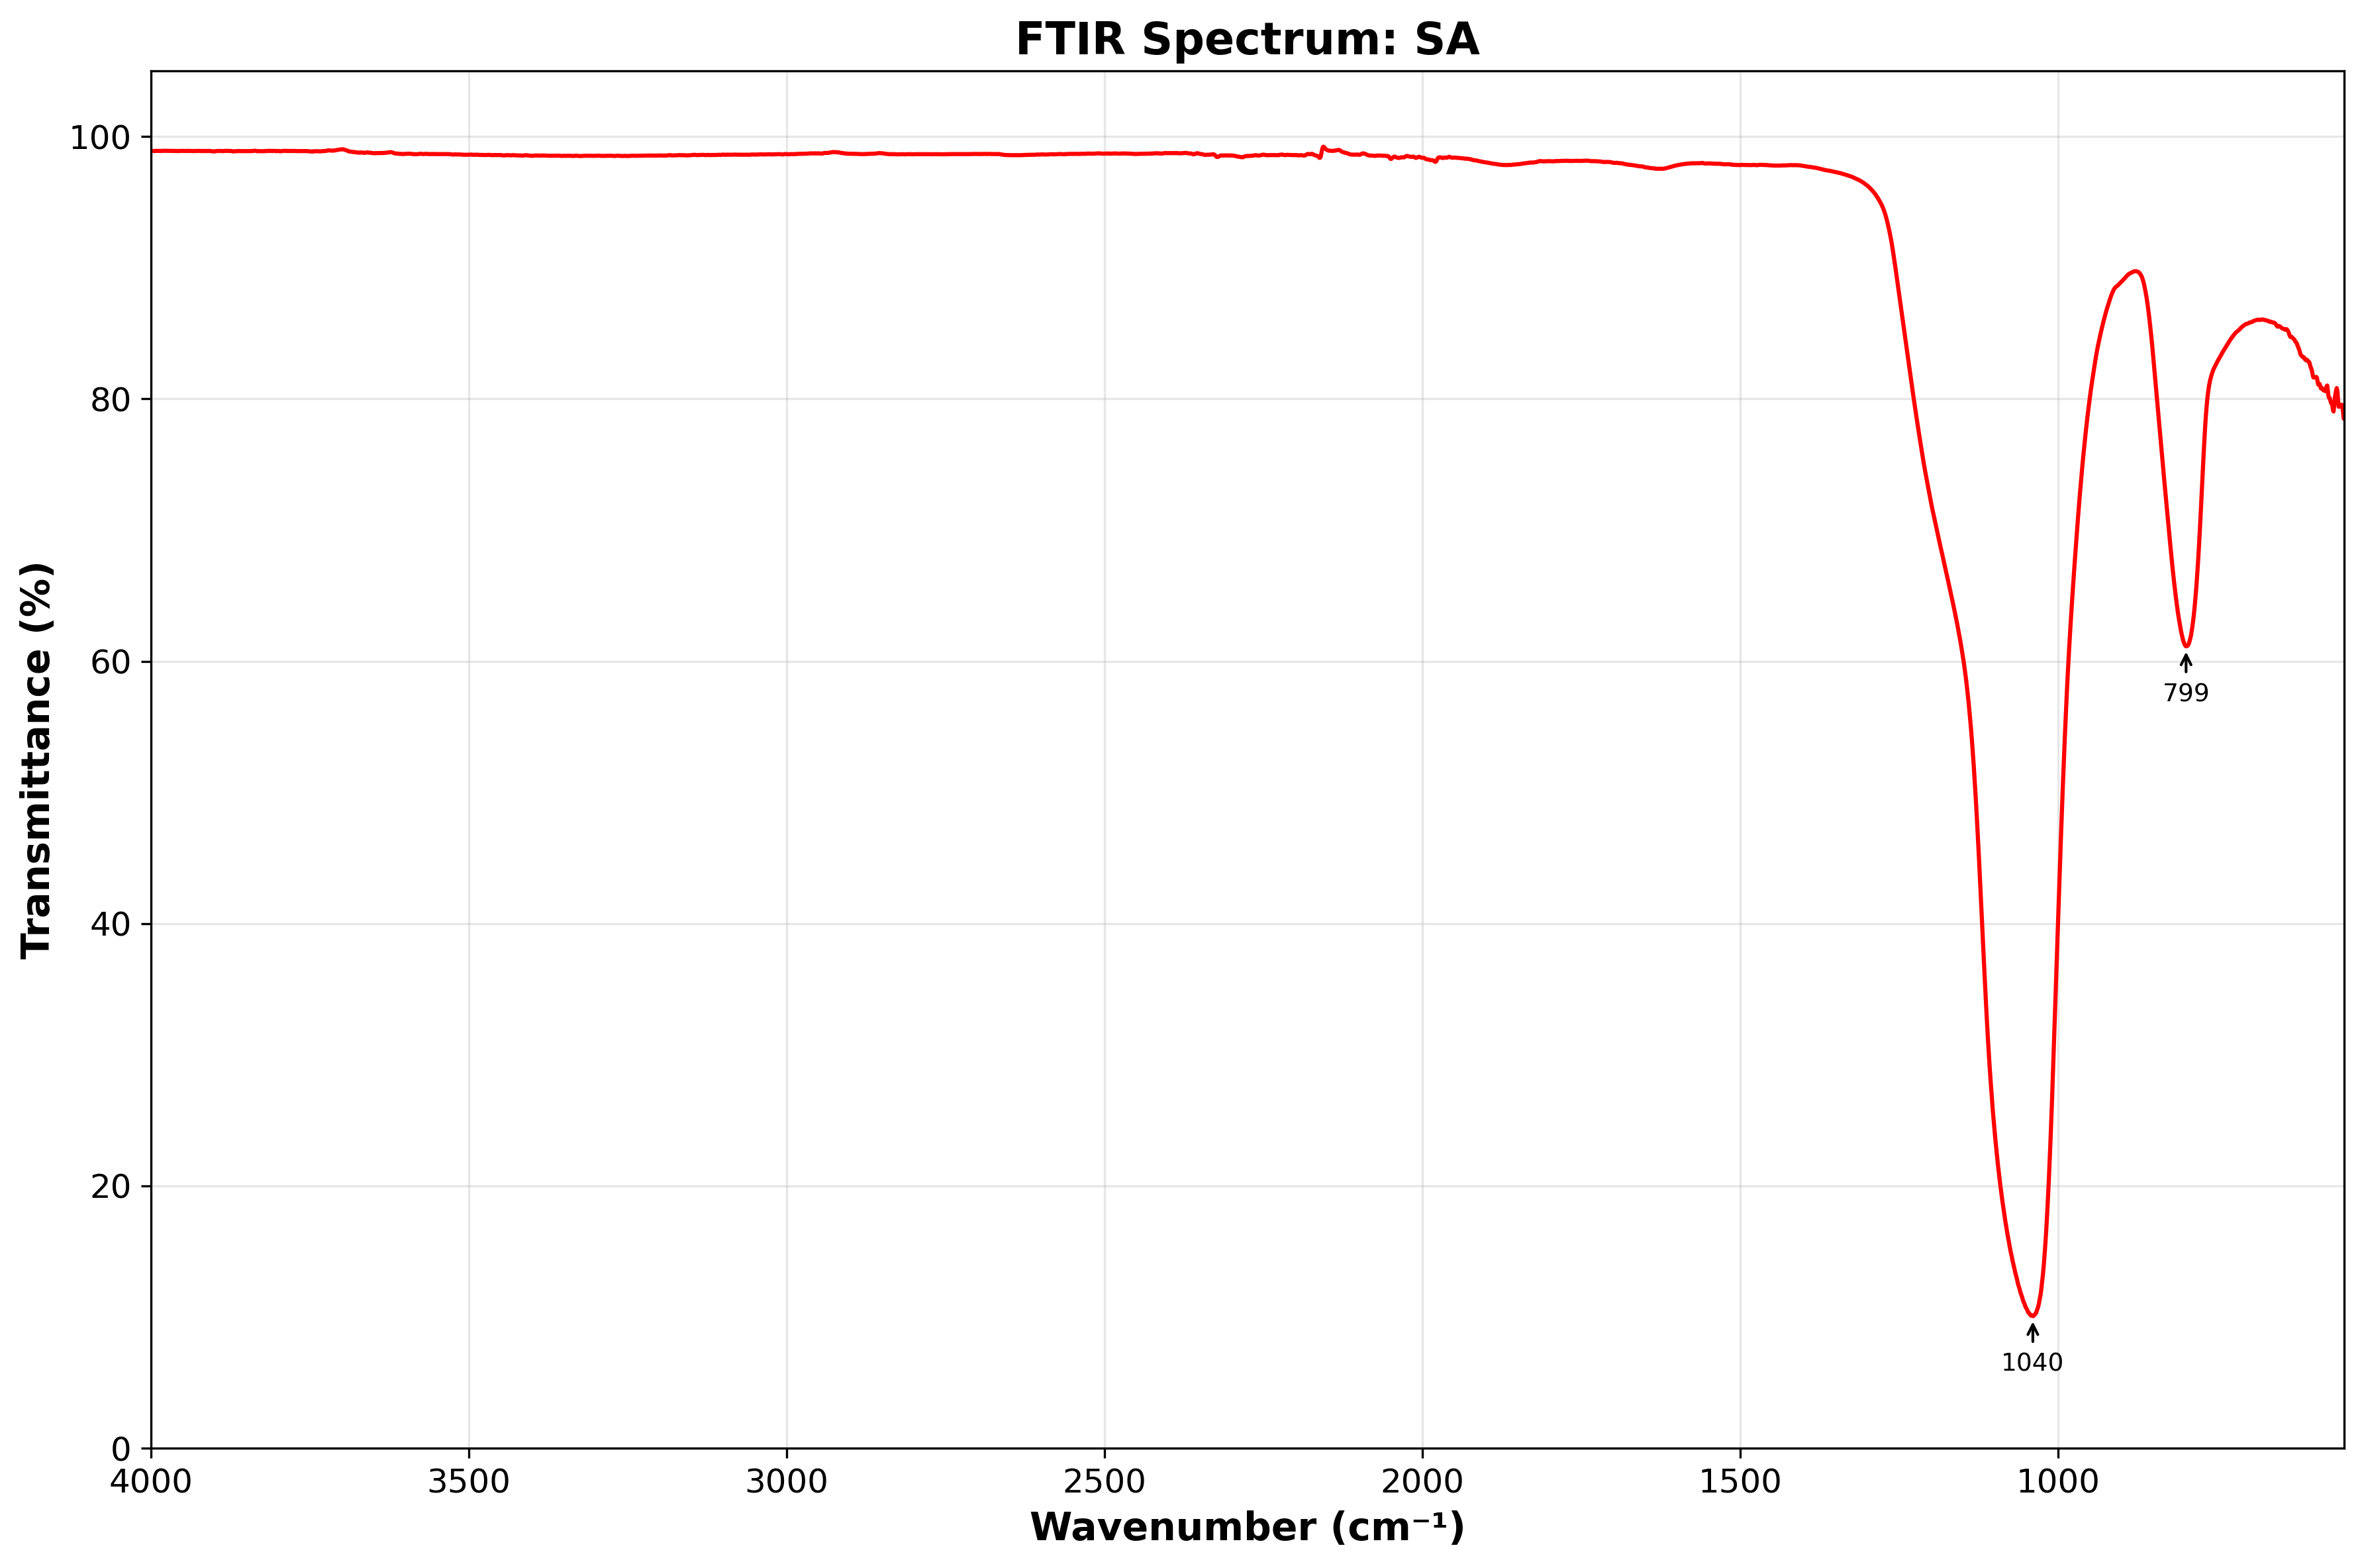
\includegraphics[width=0.475\textwidth]{Cap4/images/SA_ftir_spectrum.png}
    }
    \caption{FTIR spectra of solid precursors.}
    \label{fig:ftir_precursors}
\end{figure}

The spectral signatures of MK and SF validate their suitability as precursors for low-calcium alkali-activated system. MK serves as the primary source of both reactive Al\textsubscript{2}O\textsubscript{3} and SiO\textsubscript{2}.
Silica Fume, characterized by its amorphous nature and high SiO\textsubscript{2} content, is included primarily to adjust the overall Si/Al ratio of the system.
Both precursors possess the amorphous structure required, and their dominant high-frequency Si-O-T peaks confirm the presence of the structural units necessary to form the cross-linked N-A-S-H gel phase in the final binder \cite{Provis2014_LowCa}.

 Turning to the alkaline sources, the K\textsubscript{2}CO\textsubscript{3} exhibited peaks at 706, 879, 1061, 1360, and 3177 cm\textsuperscript{-1}.
 The bands at 879 cm\textsuperscript{-1} and 1360 cm\textsuperscript{-1} reinforce the existence of C-O bonds \cite{moraes2024scsa}.
 The broader peak at 3177 cm\textsuperscript{-1} is often attributed to O-H stretching \cite{Brito2008}, likely from adsorbed water or moisture inherent to the hygroscopic nature of the alkaline salt.
 
 Similarly, Ca(OH)\textsubscript{2} presented two primary peaks at 1435 cm\textsuperscript{-1} and 3641 cm\textsuperscript{-1}.
 The sharp peak at 3641 cm\textsuperscript{-1} is attributed to the stretching vibration of the O-H groups in portlandite, a feature noted in several studies on alkaline activated materials \cite{batista2025mgosio2}.
 The secondary, broader band observed near 1435 cm\textsuperscript{-1} is associated with the asymmetric stretching vibration of carbonate (O-C-O) bonds, specifically indicating the presence of carbonates impurities \cite{Zhao2023}.
 
 \begin{figure}[H]
     \centering
     \subfloat[Potassium Carbonate (K\textsubscript{2}CO\textsubscript{3})]{
       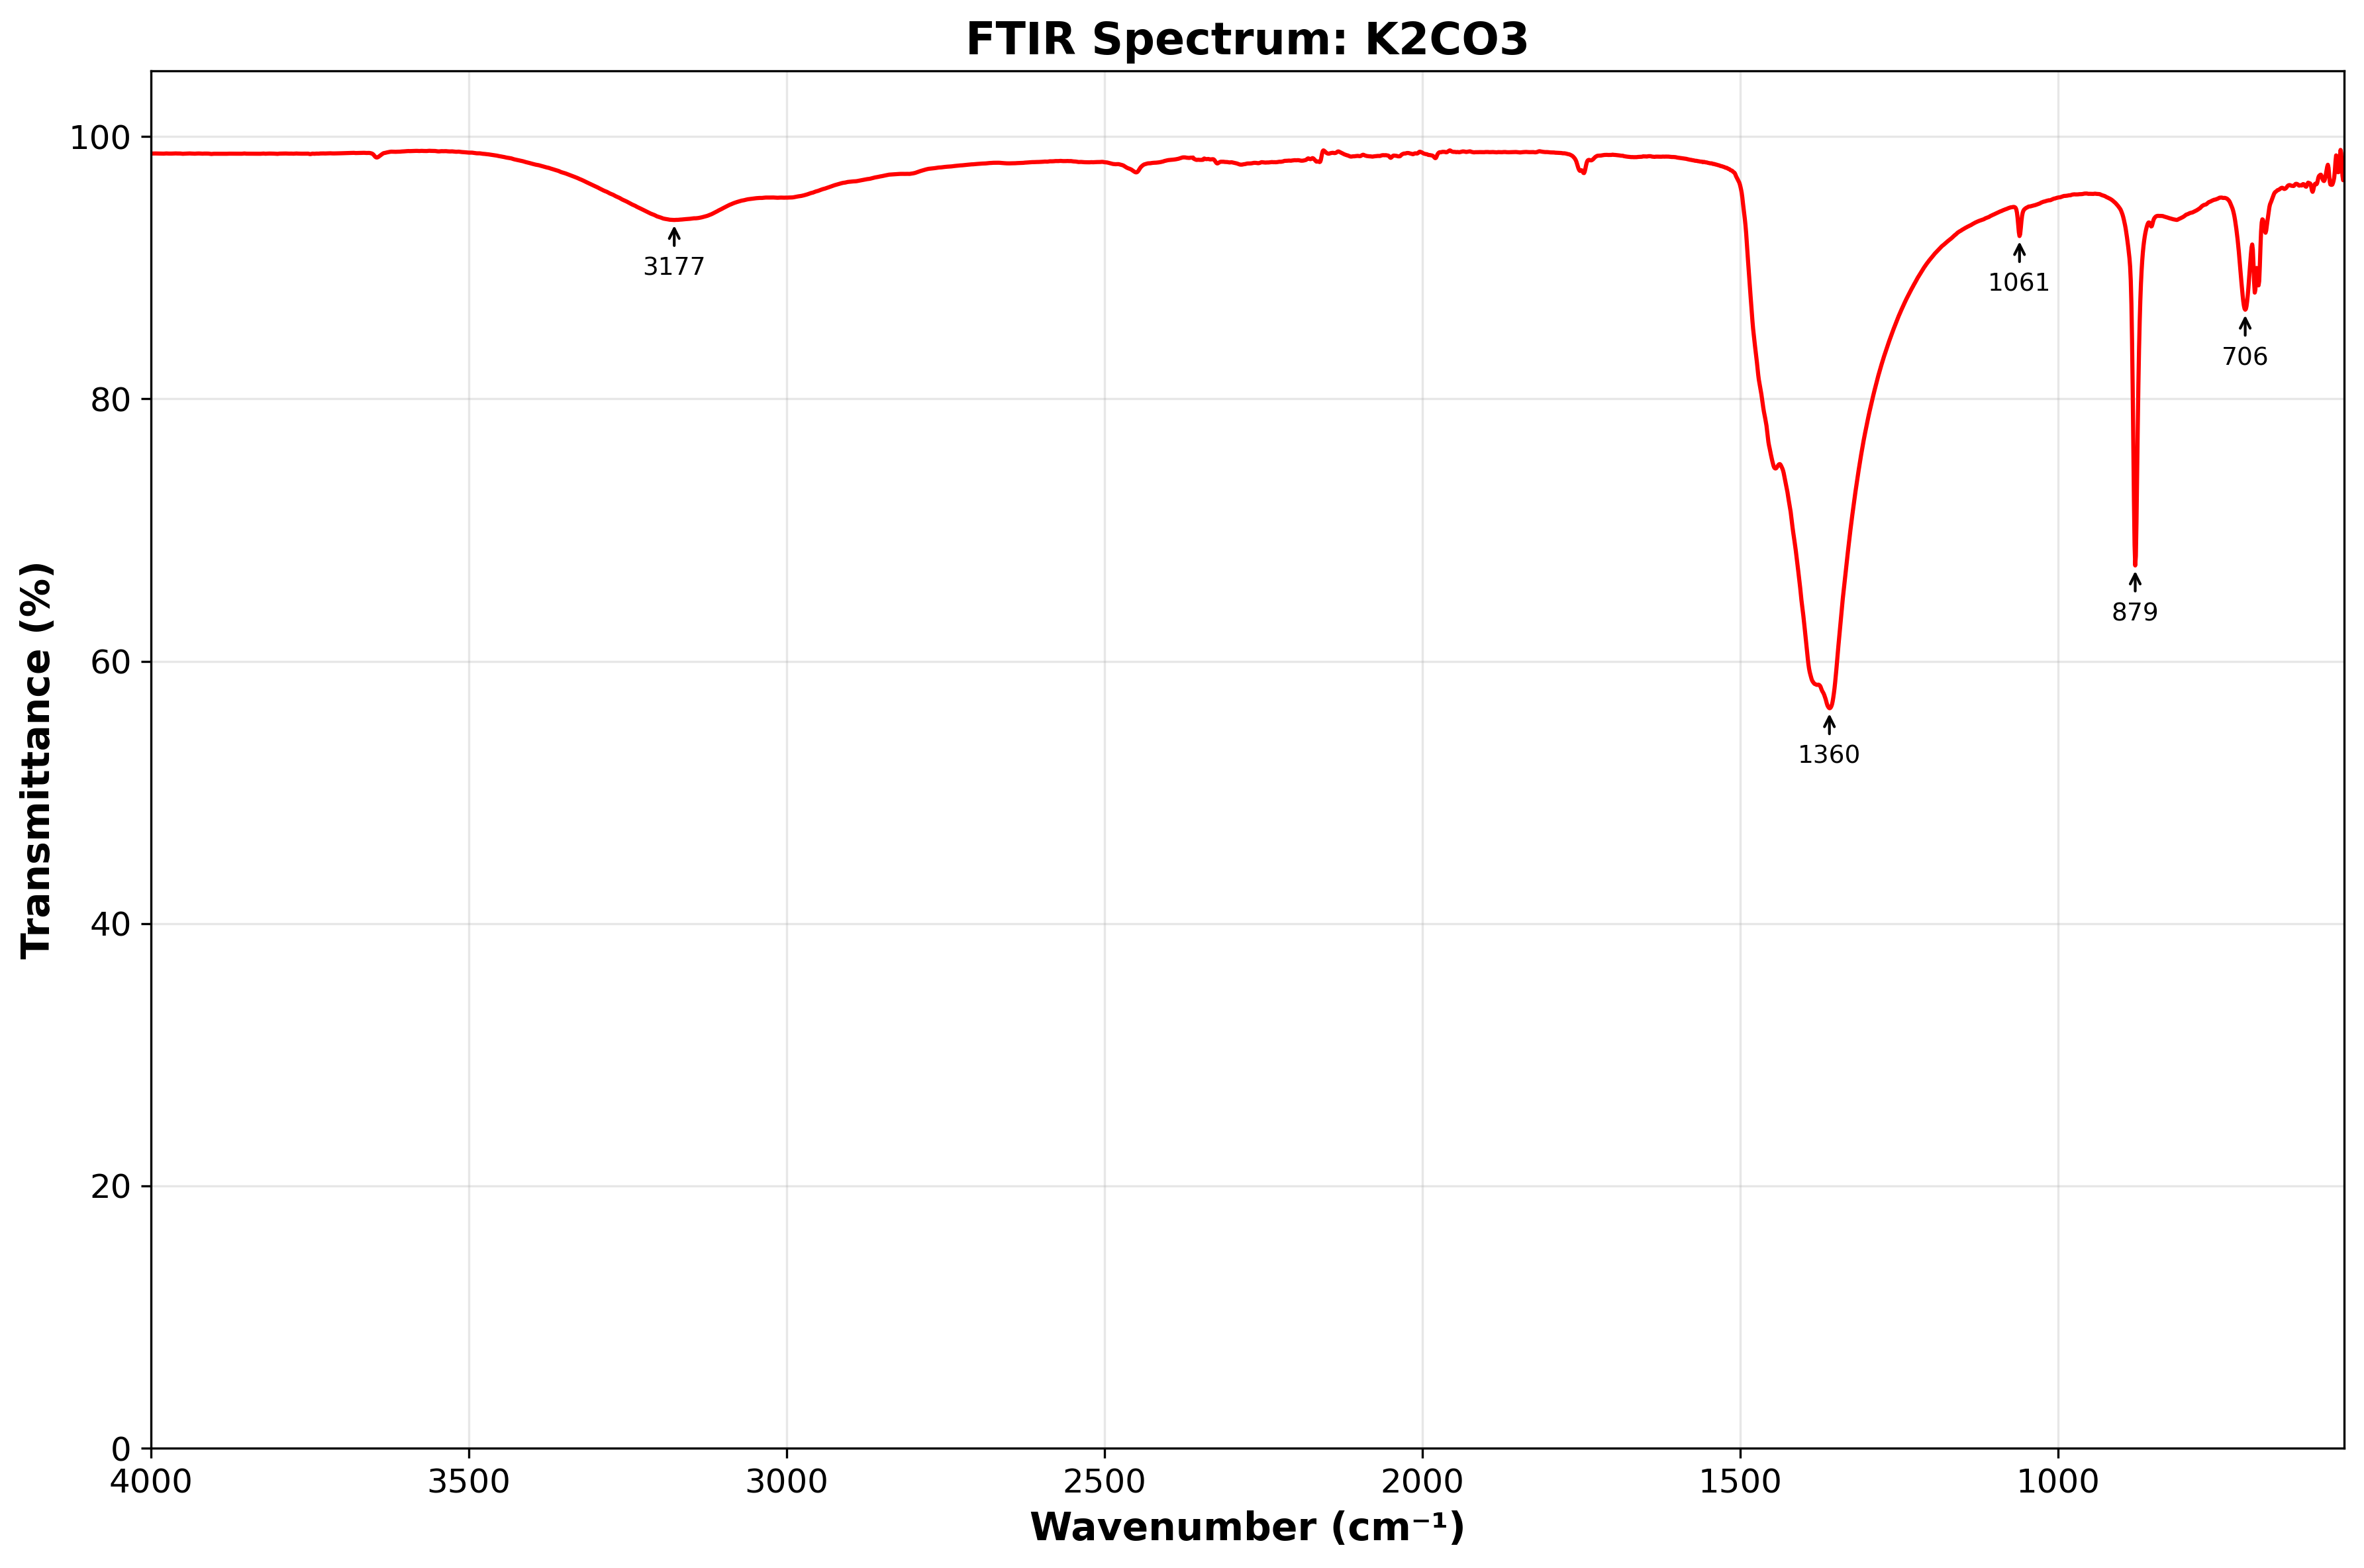
\includegraphics[width=0.475\textwidth]{Cap4/images/K2CO3_ftir_spectrum.png}
     } 
     \subfloat[Calcium Hydroxide (Ca(OH)\textsubscript{2})]{
       \includegraphics[width=0.475\textwidth]{Cap4/images/CA(OH)2_ftir_spectrum.png}
     }
     \caption{FTIR spectra of alkaline sources.}
     \label{fig:ftir_alkaline_sources}
 \end{figure}

 These results align well with existing literature concerning alkaline precursors. The carbonate peaks observed in both Ca(OH)\textsubscript{2} and K\textsubscript{2}CO\textsubscript{3} powders strongly suggest partial carbonation, a common occurrence either during handling, storage, or the sample preparation process \cite{Lei2021}.



\section{Microstructural Characterization of Pastes}

\subsection{X-Ray Diffraction}

X-ray diffraction patterns (3-day curing) of the pastes at different Si/Al ratios showed a persistent amorphous hump in all compositions, indicating the presence of aluminosilicate gel (N-A-S-H).
The hump position and shape were increasingly similar to the silica fume precursor at high Si/Al, consistent with the SEM observation, as it it shifted to the left as silica content increases. 

In agreement with other studies, the geopolymerization process—which is responsible for the strength—is indicated by the presence of the broad hump among $2\theta = 20 \approx 35\degree$.
process shifted the location of the amorphous hump to lower angles as the silica proportion increases \cite{arellano2014geopolymer,lee2017strength, wan2017geopolymerization}.

The patterns of the pastes show sharp peaks of crystalline phases of solid precursors, this indicates that the they were not involved in the geopolymerization process \cite{Geraldo2020}, but were rather present as inactive fillers, as noted by \cite{ruiz2012alkaline}.
The crystalline phases identified in the XRD patterns are presented in Table \ref{tab:xrd_phases_pastes}, showing the semi-quantitative phase composition at 3 days for different Si/Al ratios.

\begin{table}[H]
    \centering
    \caption{Semi-quantitative crystalline phases at 3 days for different Si/Al ratios (XRD).}
    \label{tab:xrd_phases_pastes}
    \begin{tabular}{lrrrrr}
        \hline
        \multirow{2}{*}{Phase (\%)} &
        \multicolumn{5}{c}{Si/Al}\\
        \cline{2-6}
        & 0.9 & 2.0 & 3.0 & 4.0 & 5.0 \\
        \hline
        Calcite (CaCO$_3$) & 77 & 56 & 43 & 52 & 79 \\
        Butschliite (K$_2$Ca(CO$_3$)$_2$) & 18 & 29 & 0 & 0 & 0 \\
        Aragonite (CaCO$_3$) & 0 & 0 & 41 & 24 & 0 \\
        Quartz (SiO$_2$) & 6 & 14 & 16 & 17 & 21 \\
        Stishovite (SiO$_2$) & 0 & 0 & 0 & 7 & 0 \\
        \hline
    \end{tabular}
\end{table}

Figure \ref{fig:xrd_pastes} exhibits that at lower Si/Al ratios, the peaks - specially from calcite - are more intense, indicating a higher presence of these crystalline phases from unreacted materials.

% Taken together, the XRD results corroborate the SEM/EDS findings: (i) all mixes formed an amorphous aluminosilicate gel, consistent with low-calcium N-A-S-H-type networks; (ii) Si/Al = 3.0 displayed the microstructurally densest matrix and, correspondingly, lower reliance on alkali-salt precipitation products; (iii) high Si/Al (4-5) retained unreacted silica, evidenced by the hump shape similarity to SF and the SiO₂ fraction; and (iv) low Si/Al (0.9) promoted alkali/carbonate crystallization (including butschliite) consistent with excess free alkali and early carbonation.

\begin{figure}[H]
    \centering
    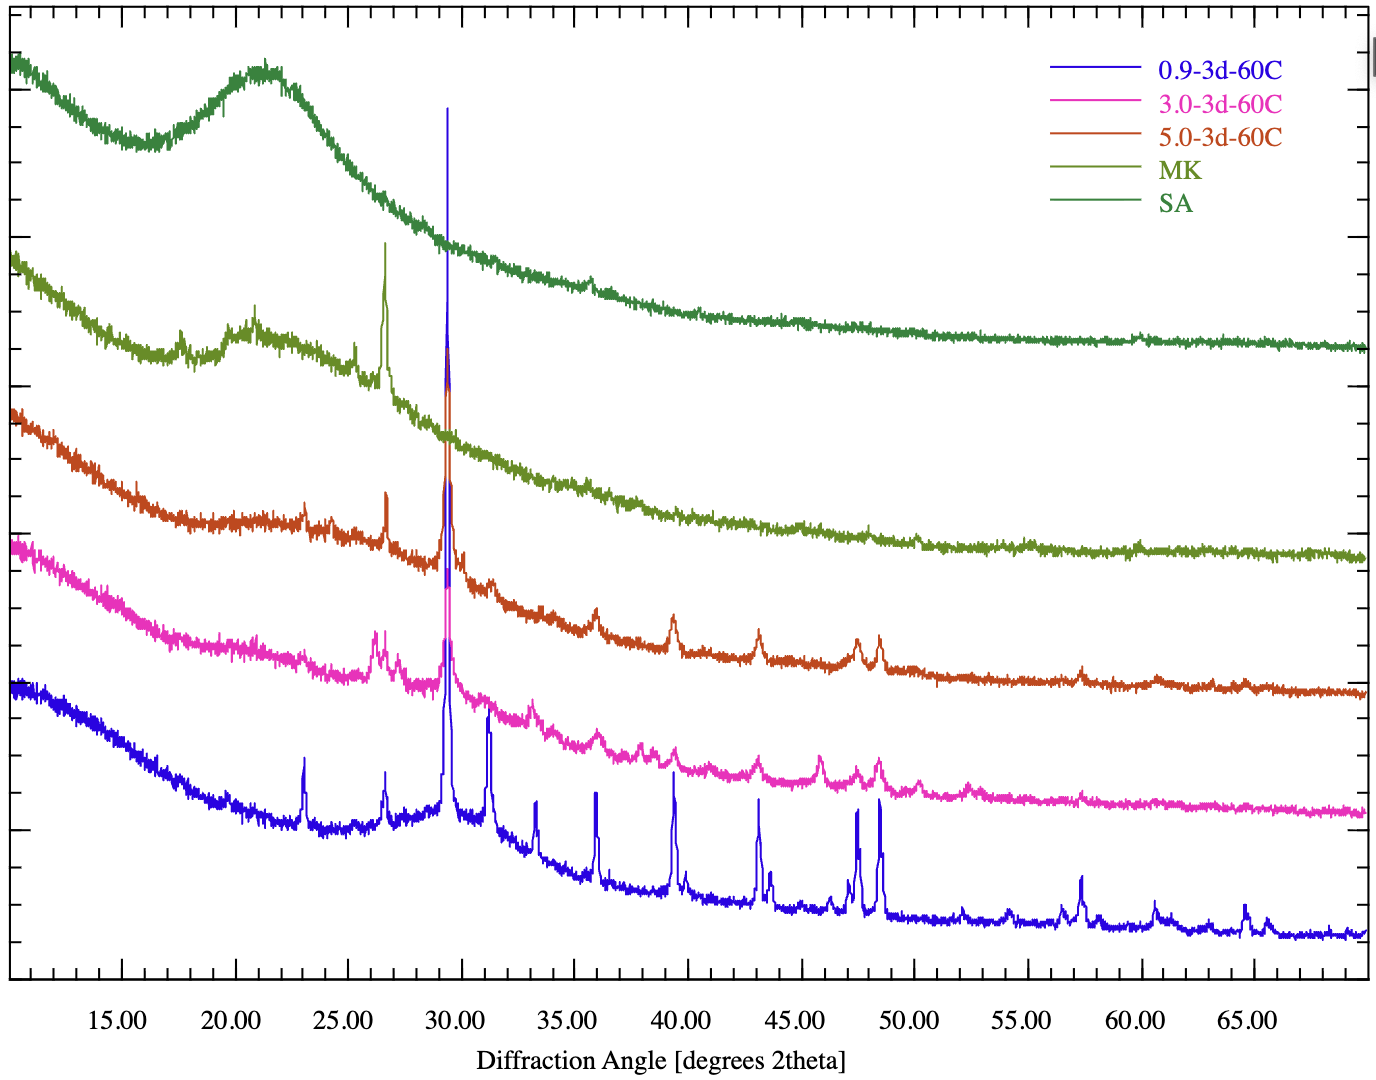
\includegraphics[width=0.8\textwidth]{Cap4/images/xrd_pastes_shifted.png}
    \caption{XRD patterns of pastes at different Si/Al ratios after 3 days of curing.}
    \label{fig:xrd_pastes}
\end{figure}

\textcolor{red}{Explain why Si/Al has stronger peaks.}

\subsection{Fourier Transform Infrared Spectroscopy}

FTIR spectra were collected for all pastes after 1 and 3 days of curing to analyze the chemical bonding and structural changes associated with geopolymerization at different Si/Al ratios.
There was no significant variation in the spectra from 1 to 3 days of curing, so only the spectra after 3 days are represented in Figure \ref{fig:ftir_pastes}.

\begin{figure}[H]
    \centering
    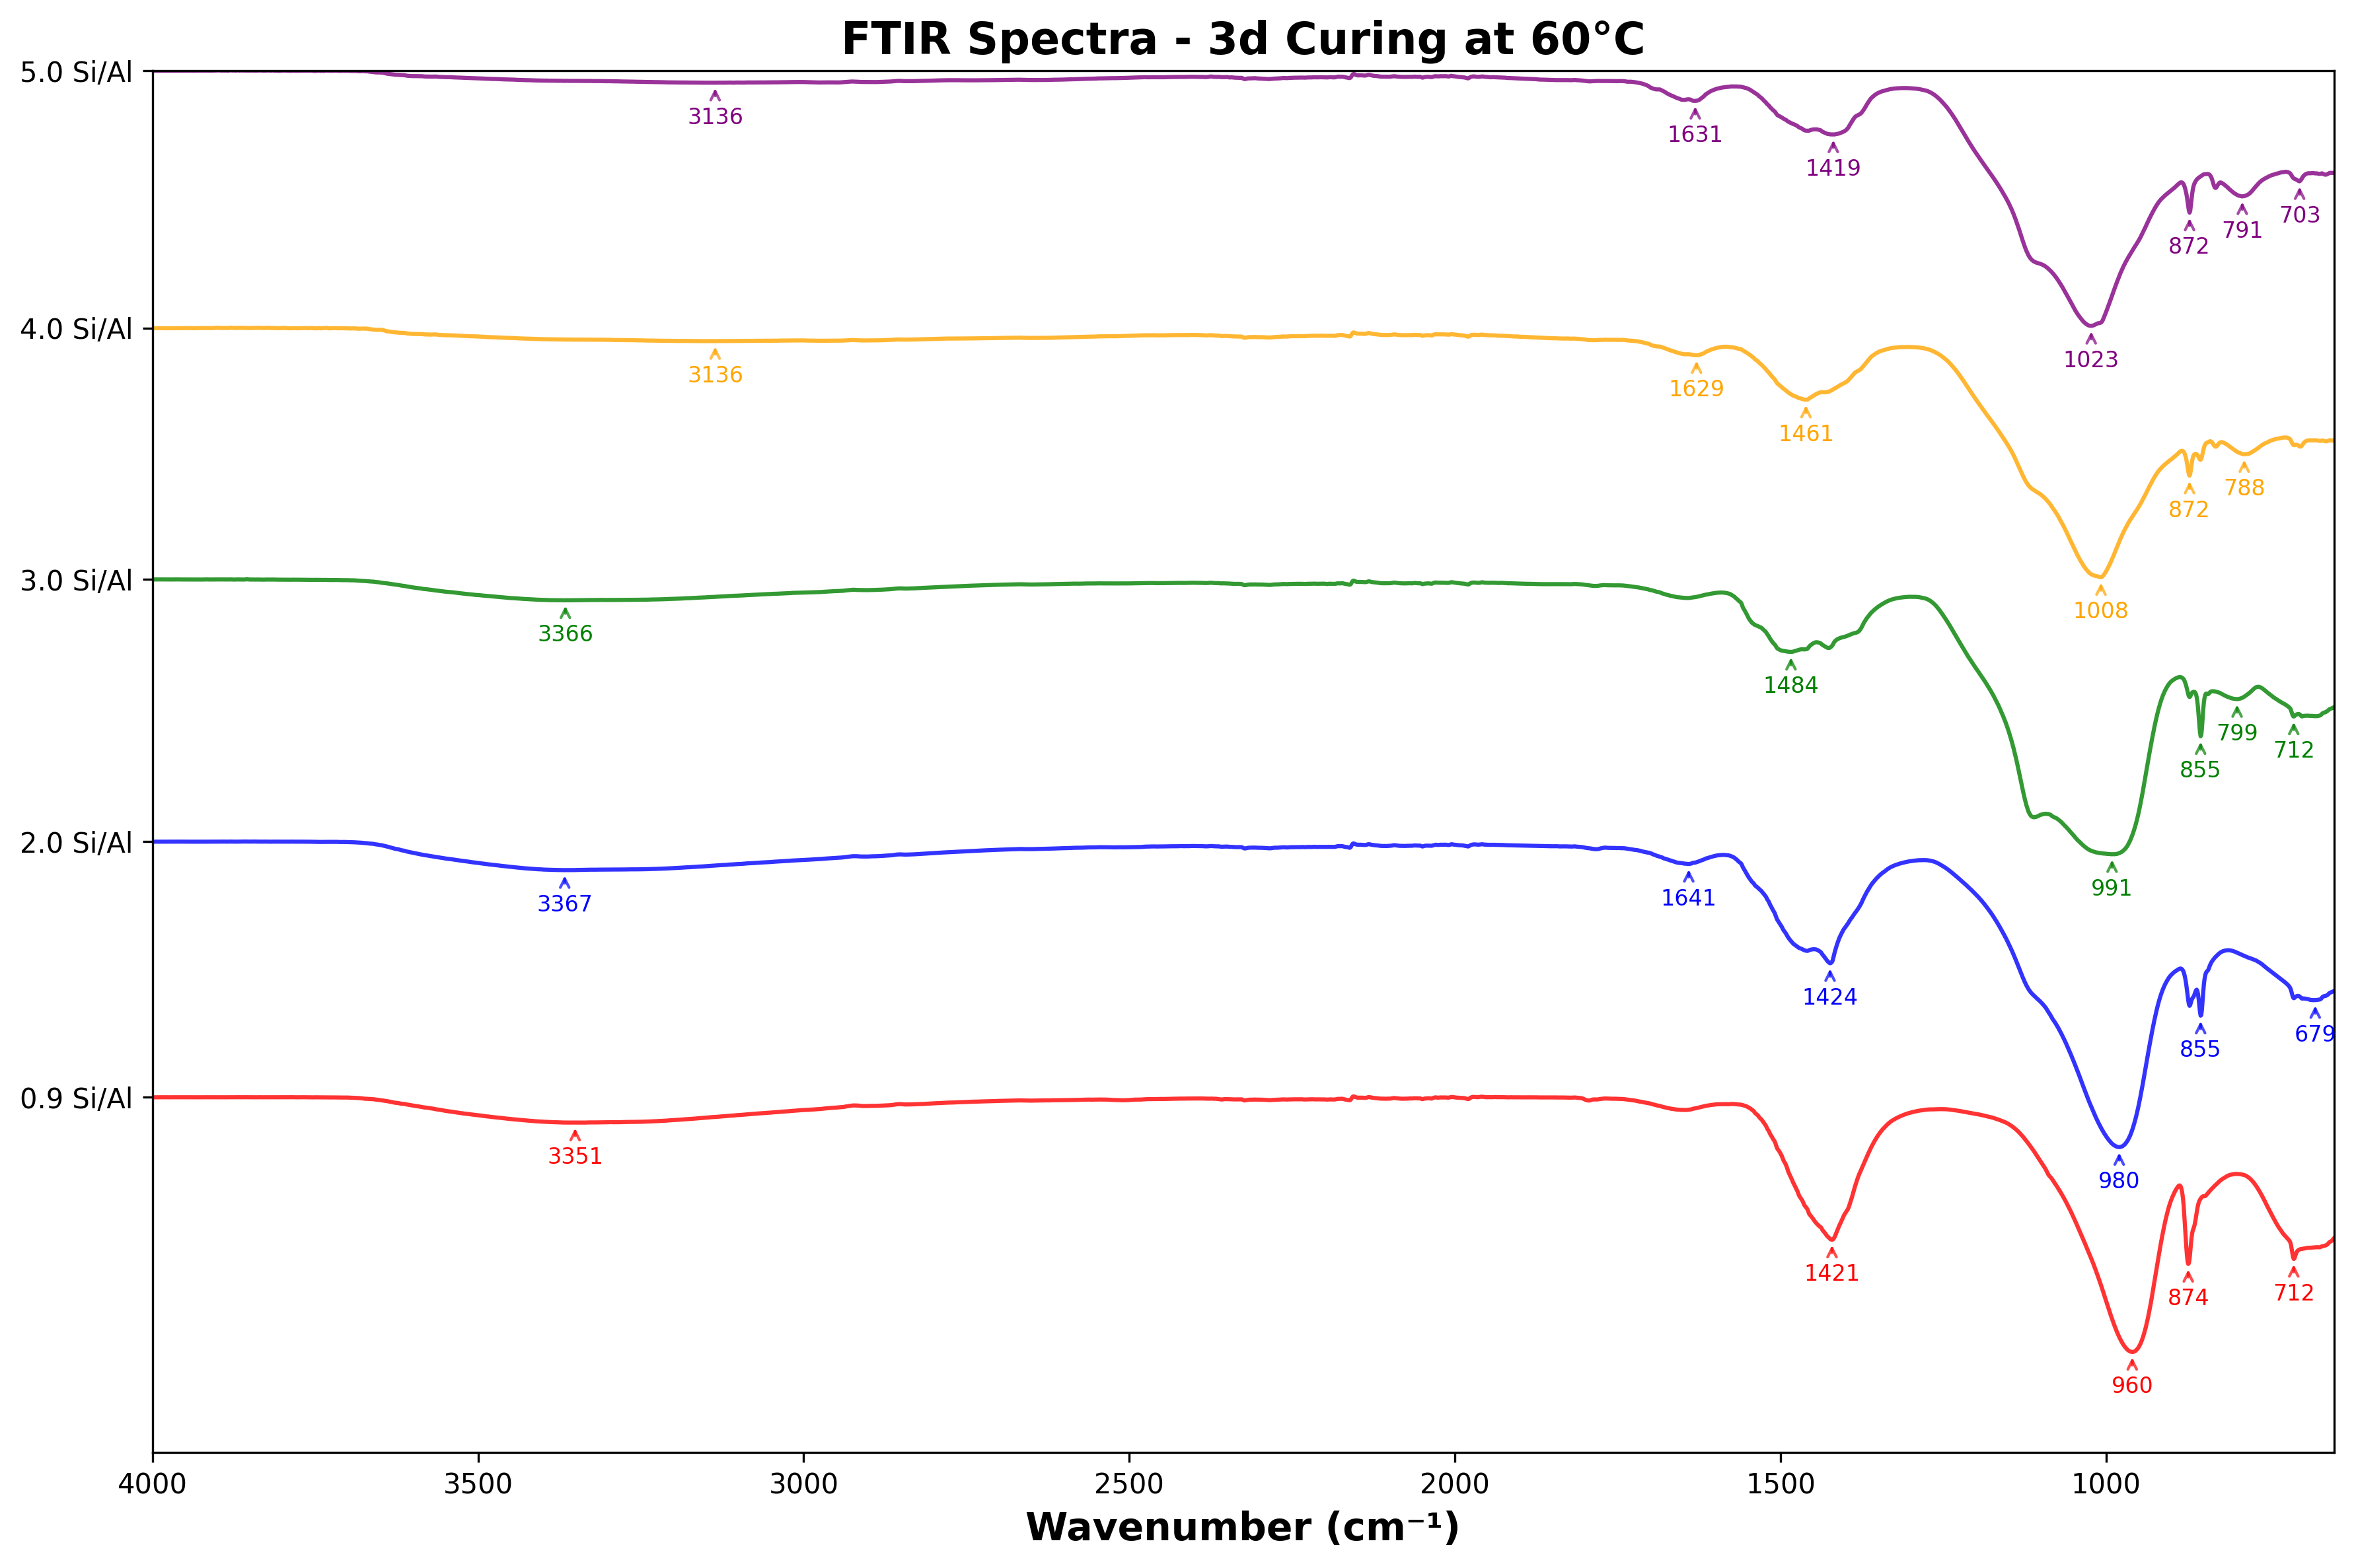
\includegraphics[width=0.8\textwidth]{Cap4/images/ftir_comparison_3d_curing.png}
    \caption{FTIR spectra of pastes at different Si/Al ratios after 3 days of curing.}
    \label{fig:ftir_pastes}
\end{figure}

The key to interpreting these spectra lies in the fingerprint region (400-1200 cm\textsuperscript{-1}), which reflects the formation of the polymeric network, and the hydroxyl/carbonate regions (1300-3700 cm\textsuperscript{-1}), which indicate water and carbonation.
The Table \ref{tab:ftir_assignments} summarizes the main FTIR peaks observed in the pastes and their assignments.

At lower Si/Al ratios, the reaction leads to a network with a higher density of Si-O-Al bonds, while the increasing Si content promotes the formation of Si-O-Si linkages, resulting in a more siliceous gel structure, shifting the main peak of Figure \ref{fig:ftir_pastes} towards higher wavenumbers, from 960 cm\textsuperscript{-1} (Si/Al = 0.9) to 1023 cm\textsuperscript{-1} (Si/Al = 5.0).
This means that the gel structure progressively replaces AlO\textsubscript{4}\textsuperscript{-} tetrahedra with SiO\textsubscript{4}\textsuperscript{-}, suggesting a higher degree of polymerization, denser and stronger molecular network \cite{pachecotorgal2014handbook}.

\begin{landscape}
    \begin{table}[p]
    \centering
    \caption{Assignment of FTIR absorption bands observed in pastes after 3 days of curing at 60$\degree$C, where T = Si or Al.}
    \vspace{0.5cm}
    {\small % Reduce font size for the table
    \renewcommand{\arraystretch}{1.2} % Increase row spacing
    \begin{tabular}{p{2.5cm} p{2.5cm} p{3cm} p{8cm} p{3cm}}
        \hline
        Wavenumber Range (cm$^{-1}$) & Observed Peaks & Vibration Mode & Chemical Significance & Reference \\
        \hline
        % 3641 & 3641 (Ca(OH)$_2$ precursor) & O-H stretching & Sharp band characteristic of crystalline portlandite (Ca(OH)$_2$). & \\
        3100-3450 & 3111, 3136, 3177, 3325, 3367 & O-H stretching & Represents weakly bonded or physically adsorbed water, and hydroxyl groups involved in hydrogen bonding within the gel structure. & \cite{Zhao2023}, \cite{provis2009geopolymers, ma2022calcium}\\
        1620-1645 & 1629, 1631, 1632, 1641 & H-O-H bending & Vibration of interlayered or physically bound water molecules in the AAM matrix. & \cite{Zhao2023}, \cite{pachecotorgal2014handbook}\\
        1350-1500 & 1419, 1423, 1461, 1484 & C-O stretching & Characteristic of carbonates, indicating atmospheric carbonation (formation of CaCO$_3$ or K$_2$CO$_3$). & \cite{Zhao2023, pachecotorgal2014handbook, moraes2024scsa}\\
        950-1100 & 960, 1008, 1023 & Si-O-T asymmetric stretching & Primary diagnostic band of N-A-S-H gel formation. Shifted to lower frequencies when compared to precursors (SF: 1040, MK: 1051 cm$^{-1}$) indicates precursor dissolution and gel polymerization. & \cite{ma2022calcium, Zhao2023, provis2009geopolymers}\\
        780-880 & 787, 855, 872 & Si-O-Si symmetric stretching or C-O bending & Peaks around 780-800 cm$^{-1}$ relate to unreacted quartz. Bands in 850-880 cm$^{-1}$ are associated with carbonate bending vibrations. & \cite{moraes2024scsa, pachecotorgal2014handbook}\\
        550-700 & 563, 679, 703, 712 & O-T-O or Al-O-T bending & Associated with bending vibrations in the tetrahedral network, specifically Al-O linkages in AlO$_4$ units or O-Si-O bending. & \cite{Zhao2023, ma2022calcium} \\
        \hline
    \end{tabular}
    }
    \label{tab:ftir_assignments}
    \end{table}
\end{landscape}

\subsection{Porosity}

The results of density determined by He gas pycnometry are presented in Table \ref{tab:he_pycnometry}.
\textcolor{red}{What is this standard deviation?}
\textcolor{red}{Explain why the density is 3.0 > 0.9 > 5.0}

\begin{table}[H]
  \centering
  \caption{Density results of the samples by He-pycnometry \label{tab:he_pycnometry}.}
  \begin{tabular}{lccc}
    \hline
    Sample & Density (g/cm$^3$) & Average Density (g/cm$^3$) & Standard Deviation \\ 
    \hline
    \multirow{5}{*}{0.9-3d-60$\degree$C} 
    & 2.1663 & \multirow{5}{*}{2.170} & \multirow{5}{*}{0.002} \\
    & 2.1715 &  &  \\
    & 2.1686 &  &  \\
    & 2.1716 &  &  \\
    & 2.1712 &  &  \\ 
    \hline
    \multirow{5}{*}{3.0-3d-60$\degree$C} 
    & 2.1846 & \multirow{5}{*}{2.184} & \multirow{5}{*}{0.002} \\
    & 2.1866 &  &  \\
    & 2.1806 &  &  \\
    & 2.1820 &  &  \\
    & 2.1843 &  &  \\ 
    \hline
    \multirow{5}{*}{5.0-3d-60$\degree$C} 
    & 2.1547 & \multirow{5}{*}{2.139} & \multirow{5}{*}{0.009} \\
    & 2.1350 &  &  \\
    & 2.1388 &  &  \\
    & 2.1345 &  &  \\
    & 2.1342 &  &  \\ 
    \hline
  \end{tabular}
\end{table}


The Table \ref{tab:mip} presents the results obtained from mercury intrusion porosimetry tests on the analyzed samples.
Figure 1 shows the mercury intrusion curves as a function of pore diameter for the samples.
\textcolor{red}{Explain that eventhough 5.0 has the smallest average diameter, 3.0 is the one with the most refined porosity, because it has more pores below 0.16 um. Does literature says anything about low Al/Si having coarser porosity?}

\begin{table}[H]
  \centering
  \caption{Results obtained from mercury intrusion porosimetry tests. \label{tab:mip}}
  % \begin{tabular}{l p{1.5cm} c p{2.25cm} p{2cm}}
  \begin{tabular}{c c c c c}
    \hline
    \multirow{2}{*}{Sample} & Porosity & 80\% of pores  & Average diameter & Penetration  \\ 
    & (\%) & ($\mu$m) & ($\mu$m) & (cm$^3$/g) \\
    \hline
    0.9-3d-60$\degree$C & 42.51 & Between 0.7 and 0.25 & 0.625 & 0.34 \\
    3.0-3d-60$\degree$C & 42.82 & Between 0.16 and 0.0051 & 0.12 & 0.34 \\
    5.0-3d-60$\degree$C & 46.71 & Between 1.75 and 0.065 & 0.097 & 0.40 \\
    \hline
  \end{tabular}
\end{table}

\begin{figure}[H]
  \centering
  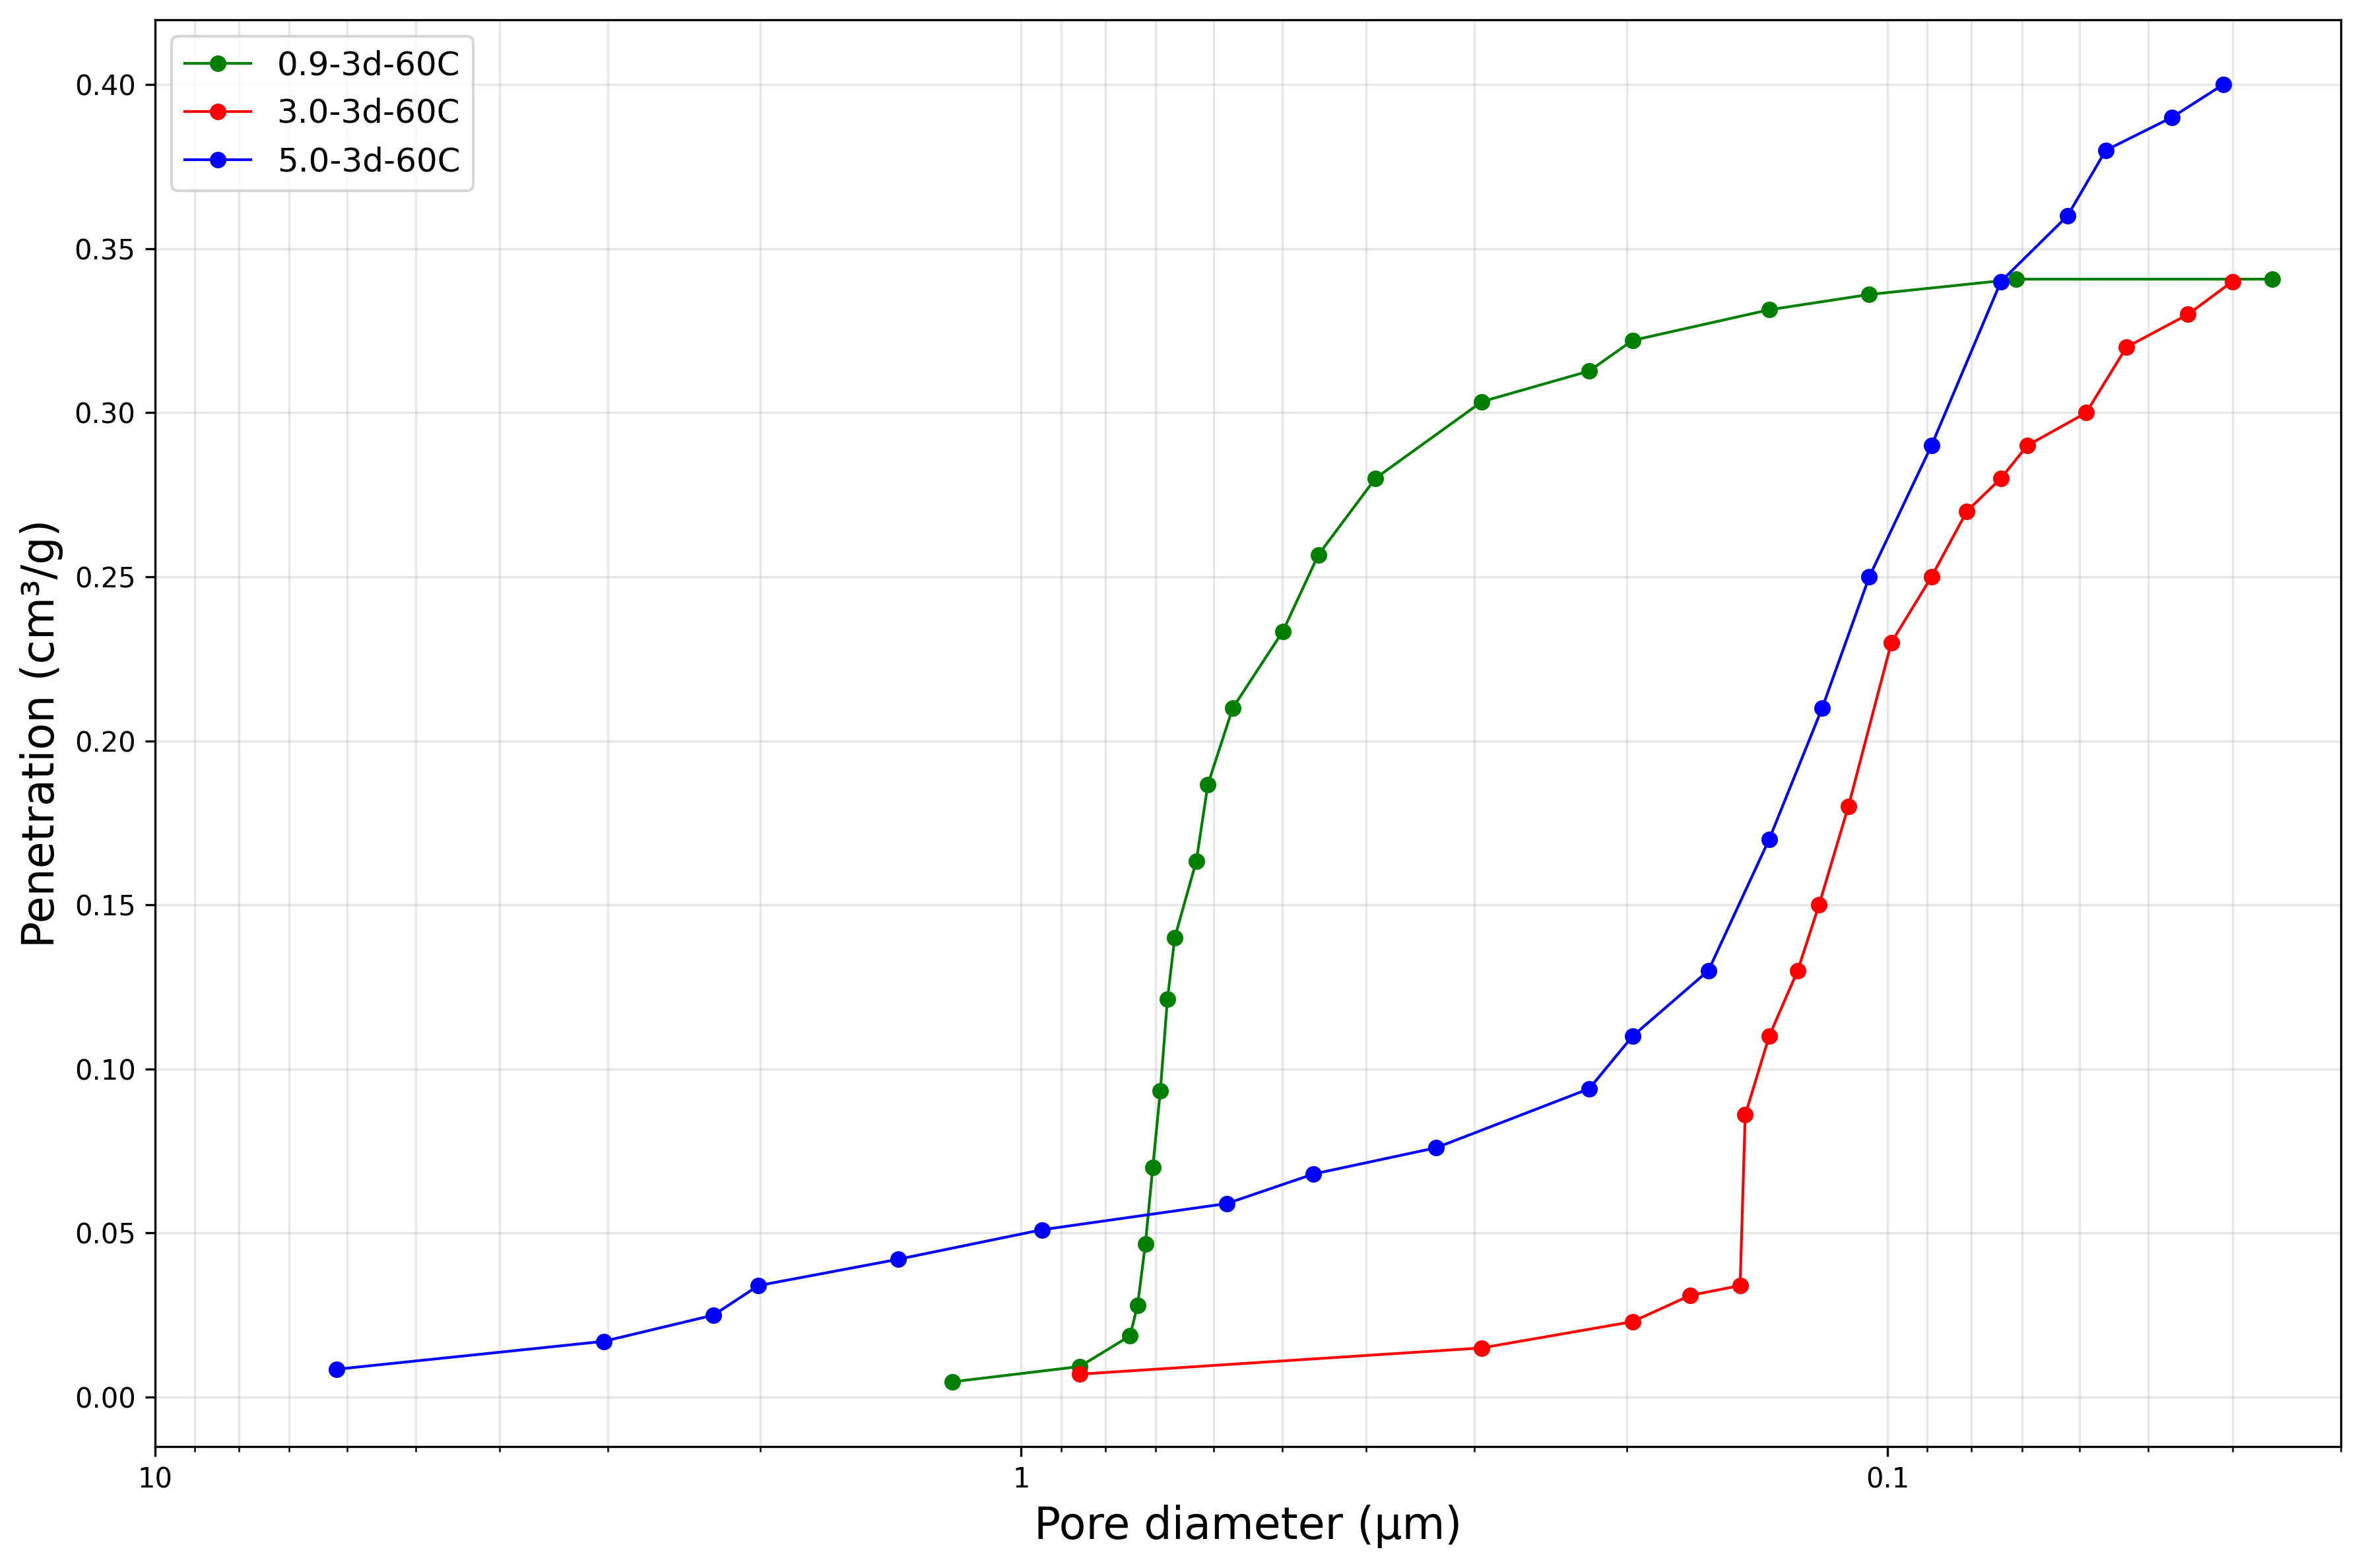
\includegraphics[width=0.75\textwidth]{Cap4/images/mip_inverted.png}
  \caption{Mercury intrusion curves as a function of pore diameter for the samples.}
  \label{fig:mip}
\end{figure}

\subsection{Scanning Electron Microscopy and Energy Dispersive Spectroscopy}

Scanning electron microscopy of the pastes cured for 3 days revealed a clear dependence of matrix morphology on the Si/Al molar ratio.
At Si/Al ratio of 0.9, the SEM images of the paste showed a higher frequency of visibly unreacted precursor particles, together with needle-shaped crystalline features and larger pores. Those unreacted particles are likely some alkali carbonate products that precipitate when mobile alkalis are not fully incorporated into the aluminosilicate gel and subsequently react with atmospheric CO\textsubscript{2} \cite{provis2018alkali}.

\begin{figure}[H]
  \centering
  \subfloat[1000× magnification]{
    
\includegraphics[width=0.4\textwidth]{Cap4/images/si_al_0-9_spot5_1000x.png}
    \label{fig:si_al_0-9_spot5_1000x}
  }
%   \hfill
  \subfloat[5000× magnification]{
    
\includegraphics[width=0.4\textwidth]{Cap4/images/si_al_0-9_spot5_5000x.png}
    \label{fig:si_al_0-9_spot5_5000x}
  }
  \caption{SEM micrographs of paste with Si/Al = 0.9 after 3 days of curing (spot 5).}
  \label{fig:si_al_0-9_spot5}
\end{figure}

By contrast, the Si/Al ratio of 3.0 paste exhibited the densest and most homogeneous matrix, with fewer discernible unreacted particles and a more continuous binder phase.
This indicates that intermediate Si/Al values promote better network polymerization and denser structure.

\begin{figure}[H]
  \centering
  \subfloat[1000× magnification]{
    
\includegraphics[width=0.4\textwidth]{Cap4/images/si_al_3-0_spot3_1000x.png}
    \label{fig:si_al_3-0_spot3_1000x}
  }
%   \hfill
  \subfloat[5000× magnification]{
    
\includegraphics[width=0.4\textwidth]{Cap4/images/si_al_3-0_spot3_5000x.png}
    \label{fig:si_al_3-0_spot3_5000x}
  }
  \caption{SEM micrographs of paste with Si/Al = 3.0 after 3 days of curing (spot 3).}
  \label{fig:si_al_3-0_spot3_sem}
\end{figure}

At Si/Al = 5.0, the SEM images showed residual spherical particles characteristic of silica fume that were not fully reacted after the curing time, indicating that at very high Si/Al the silica supply exceeds the polymerization capacity of the system.


\begin{figure}[H]
  \centering
  \subfloat[1000× magnification]{
    
\includegraphics[width=0.4\textwidth]{Cap4/images/si_al_5-0_spot1_1000x.png}
    \label{fig:si_al_5-0_spot1_1000x}
  }
%   \hfill
  \subfloat[5000× magnification]{
    
\includegraphics[width=0.4\textwidth]{Cap4/images/si_al_5-0_spot1_5000x.png}
    \label{fig:si_al_5-0_spot1_5000x}
  }
  \caption{SEM micrographs of paste with Si/Al = 5.0 after 3 days of curing (spot 1).}
  \label{fig:si_al_5-0_spot1_sem}
\end{figure}

The remaining pictures from SEM analysis are presented in Appendix \ref{appendix:sem_images}.

Energy dispersive spectroscopy was performed at representative gel regions and crystalline features observed in the SEM images.

\begin{figure}[H]
    \centering
    \subfloat[EDS layered image]{
        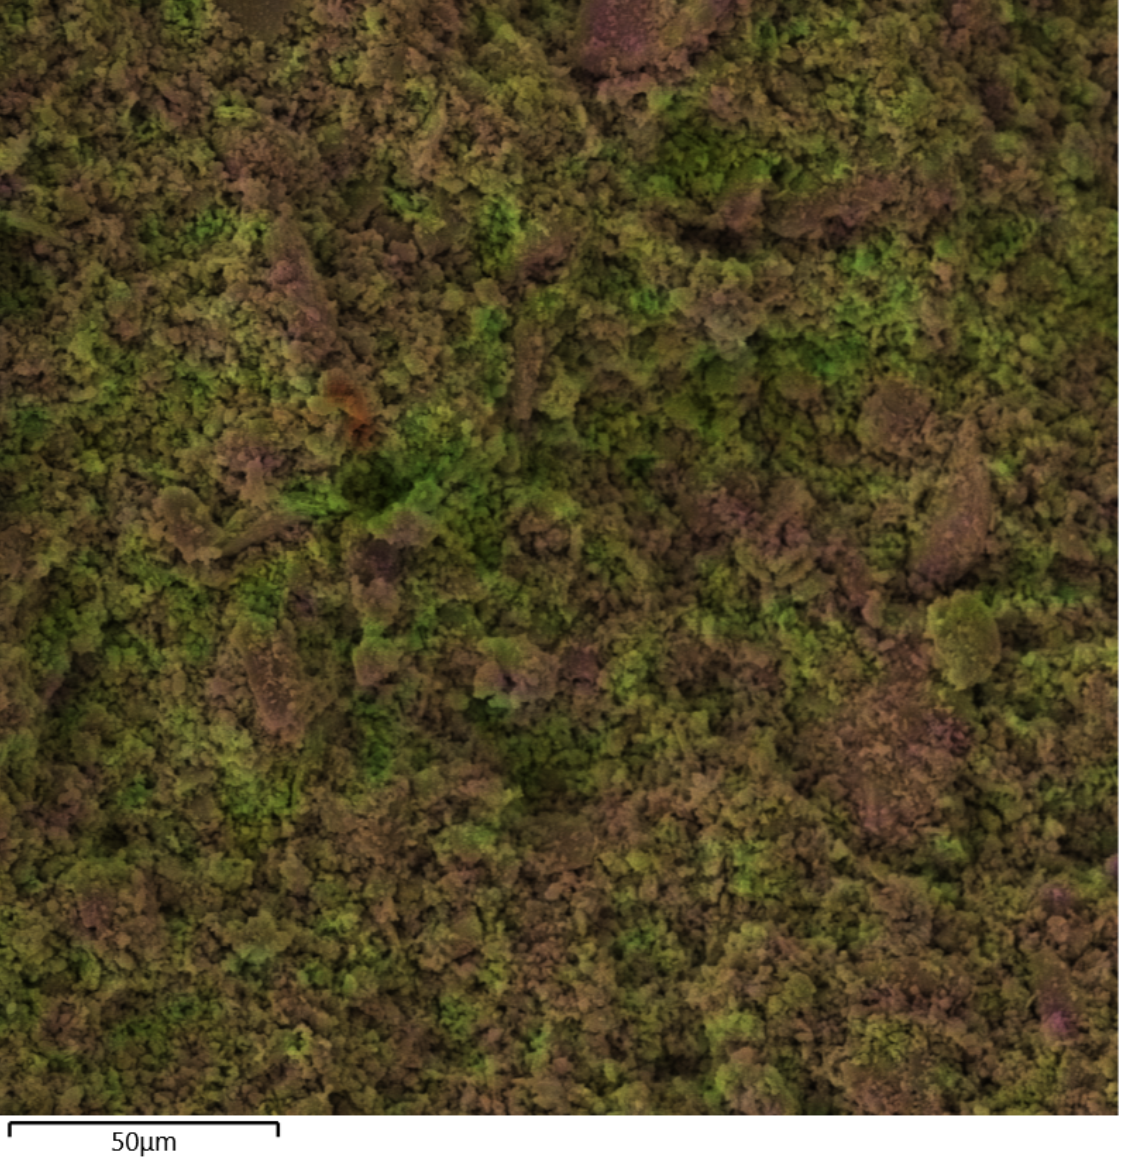
\includegraphics[height=6cm]{Cap4/images/0-9-60C-3d-Spot 5 - layered.png}
    }
    \hfill
    \subfloat[EDS map]{
        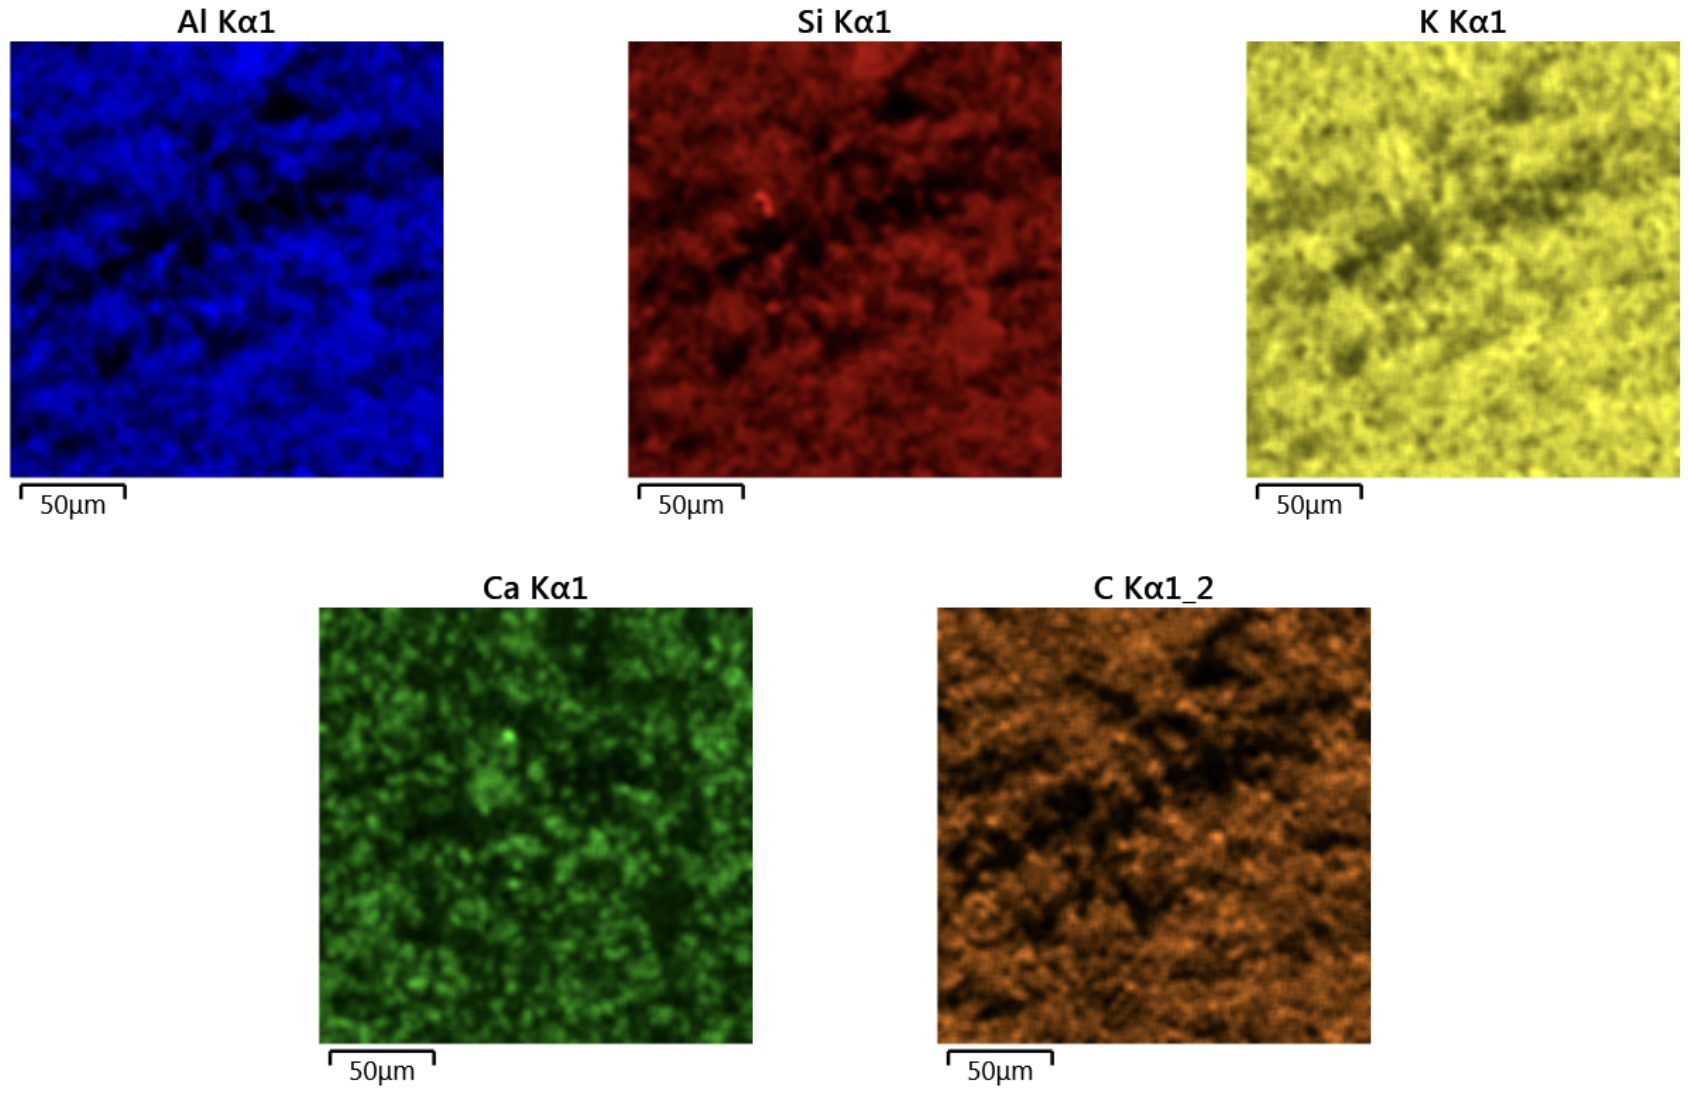
\includegraphics[height=6cm]{Cap4/images/0-9-60C-3d-Spot 5 - map.png}
    }
    \caption{EDS analysis of Spot 5, Si/Al = 0.9, cured for 3 days at 60°C at 1000× magnification.}
    \label{fig:eds_spot5_0-9}
\end{figure}

\begin{figure}[H]
    \centering
    \subfloat[EDS layered image]{
        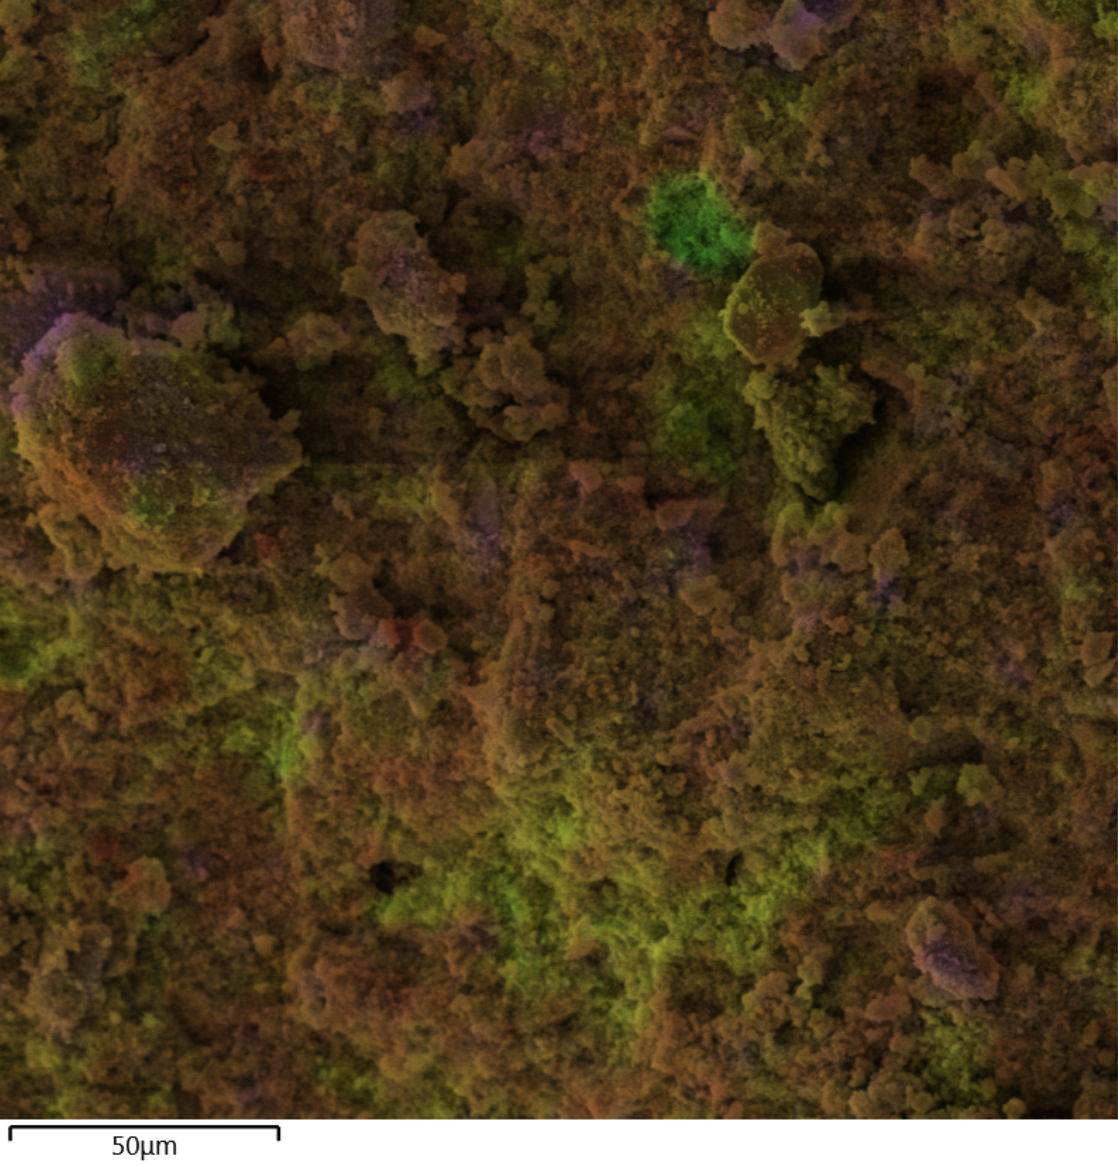
\includegraphics[height=6cm]{Cap4/images/3-0-60C-3d-Spot 3 - layered.png}
    }
    \hfill
    \subfloat[EDS map]{
        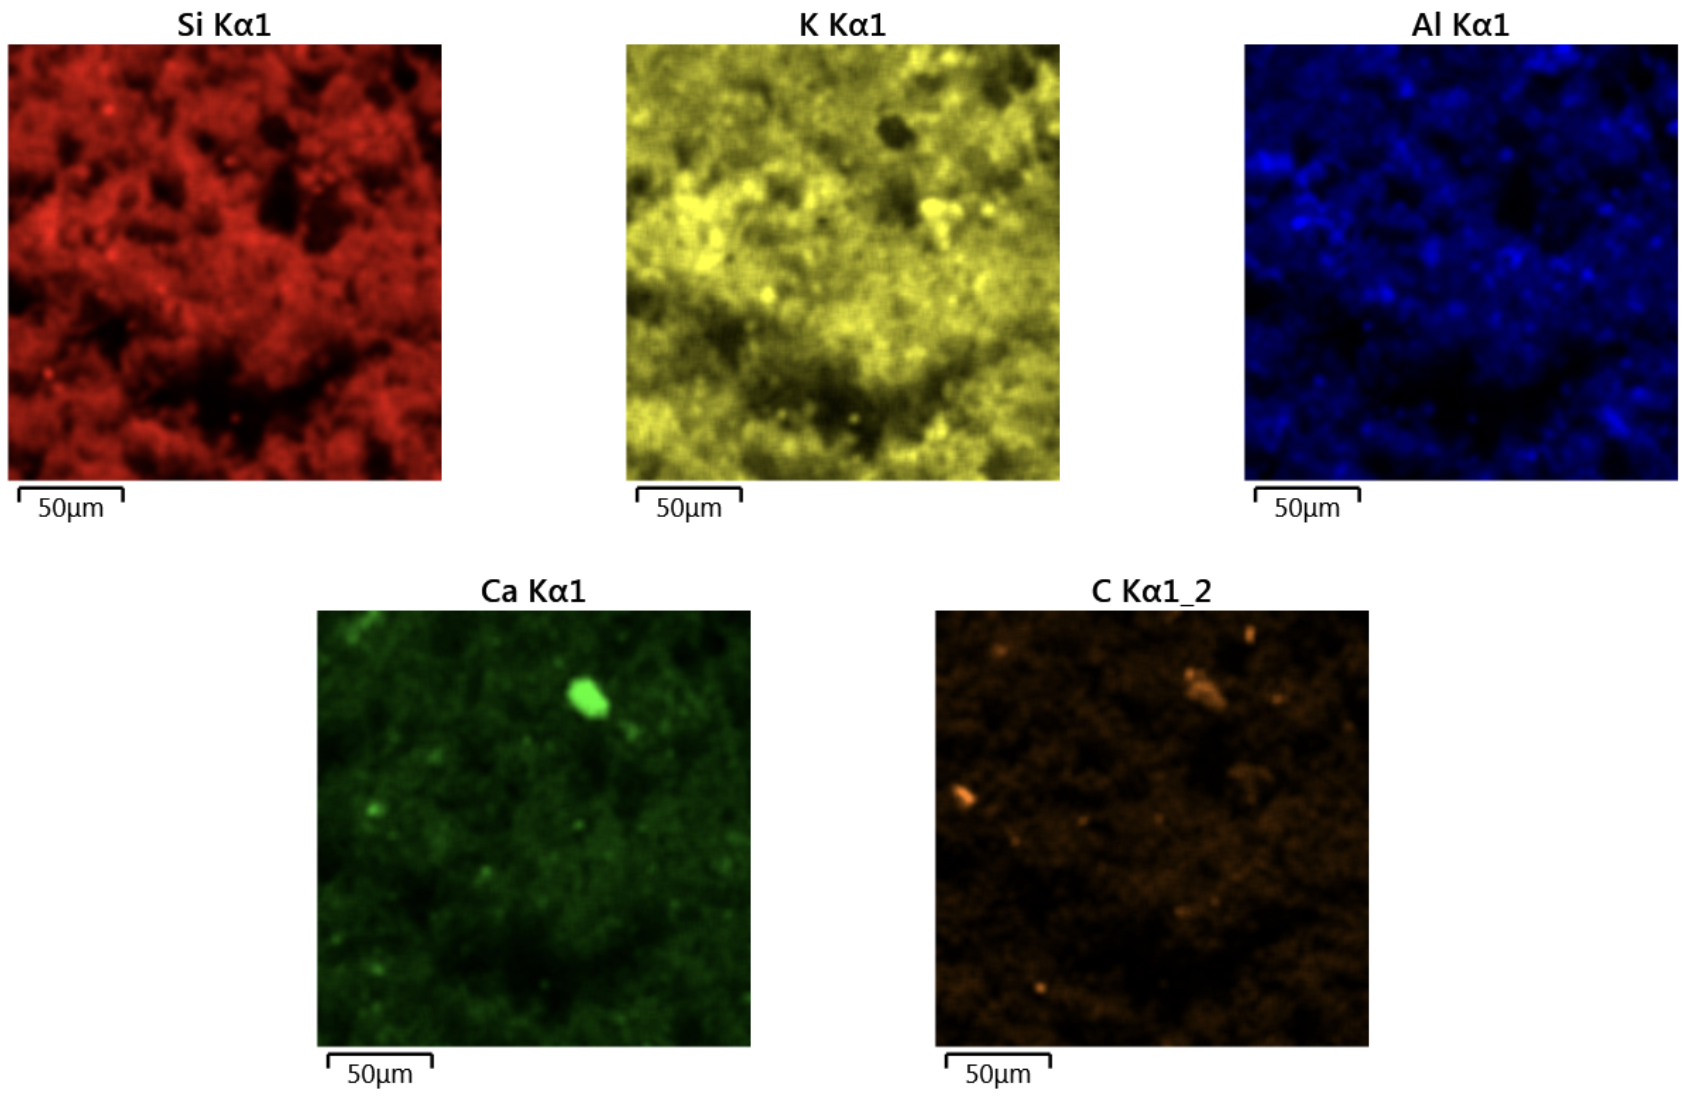
\includegraphics[height=6cm]{Cap4/images/3-0-60C-3d-Spot 3 - map.png}
    }
    \caption{EDS analysis of Spot 3, Si/Al = 3.0, cured for 3 days at 60°C at 1000× magnification.}
    \label{fig:eds_spot3_3-0}
\end{figure}

\begin{figure}[H]
    \centering
    \subfloat[EDS layered image]{
        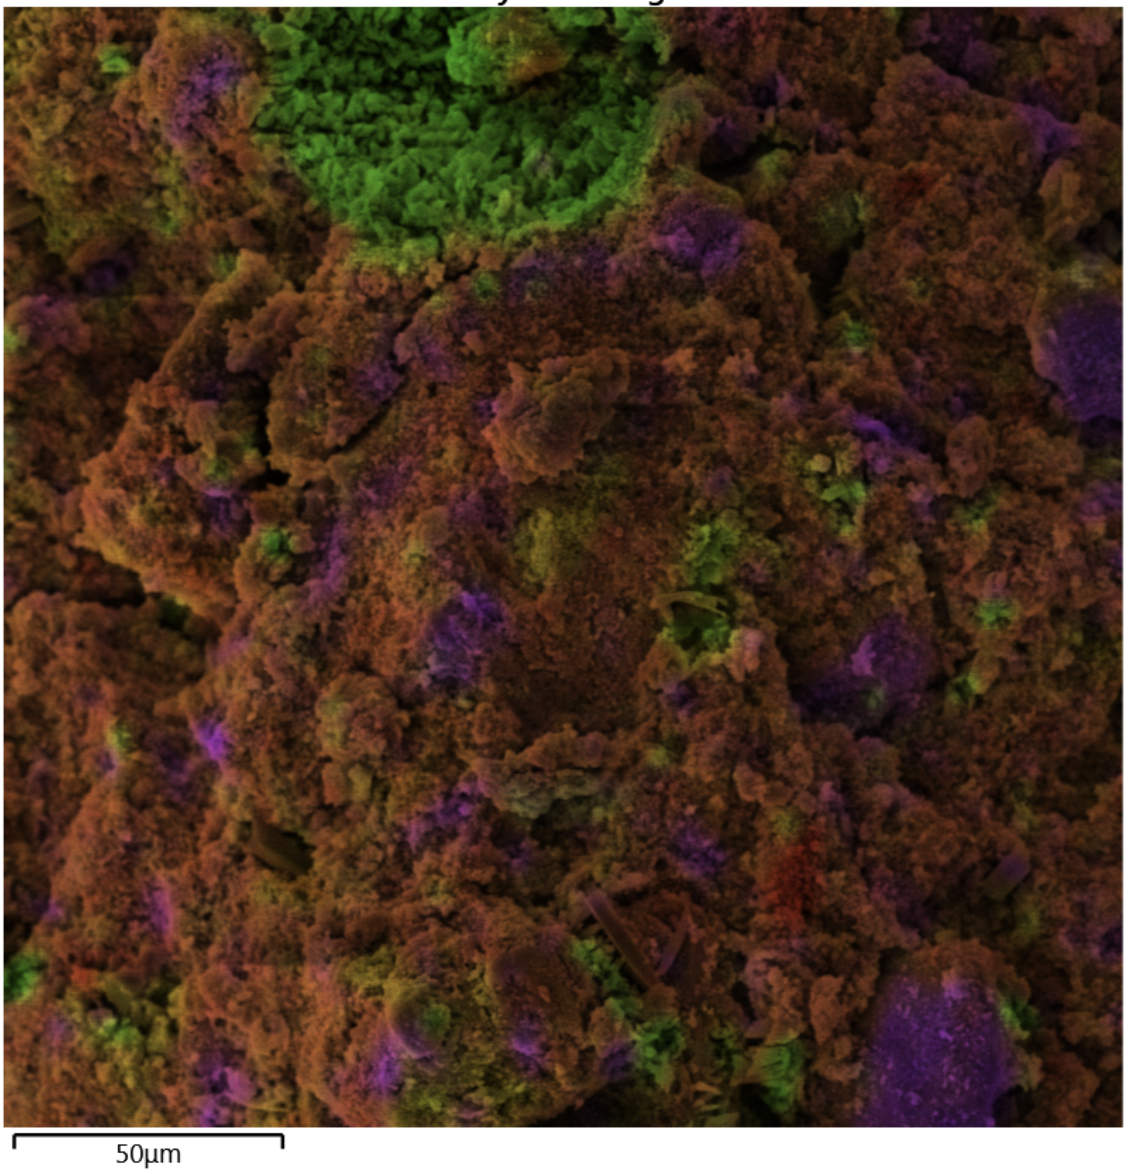
\includegraphics[height=6cm]{Cap4/images/5-0-60C-3d-Spot 1 - layered.png}
    }
    \hfill
    \subfloat[EDS map]{
        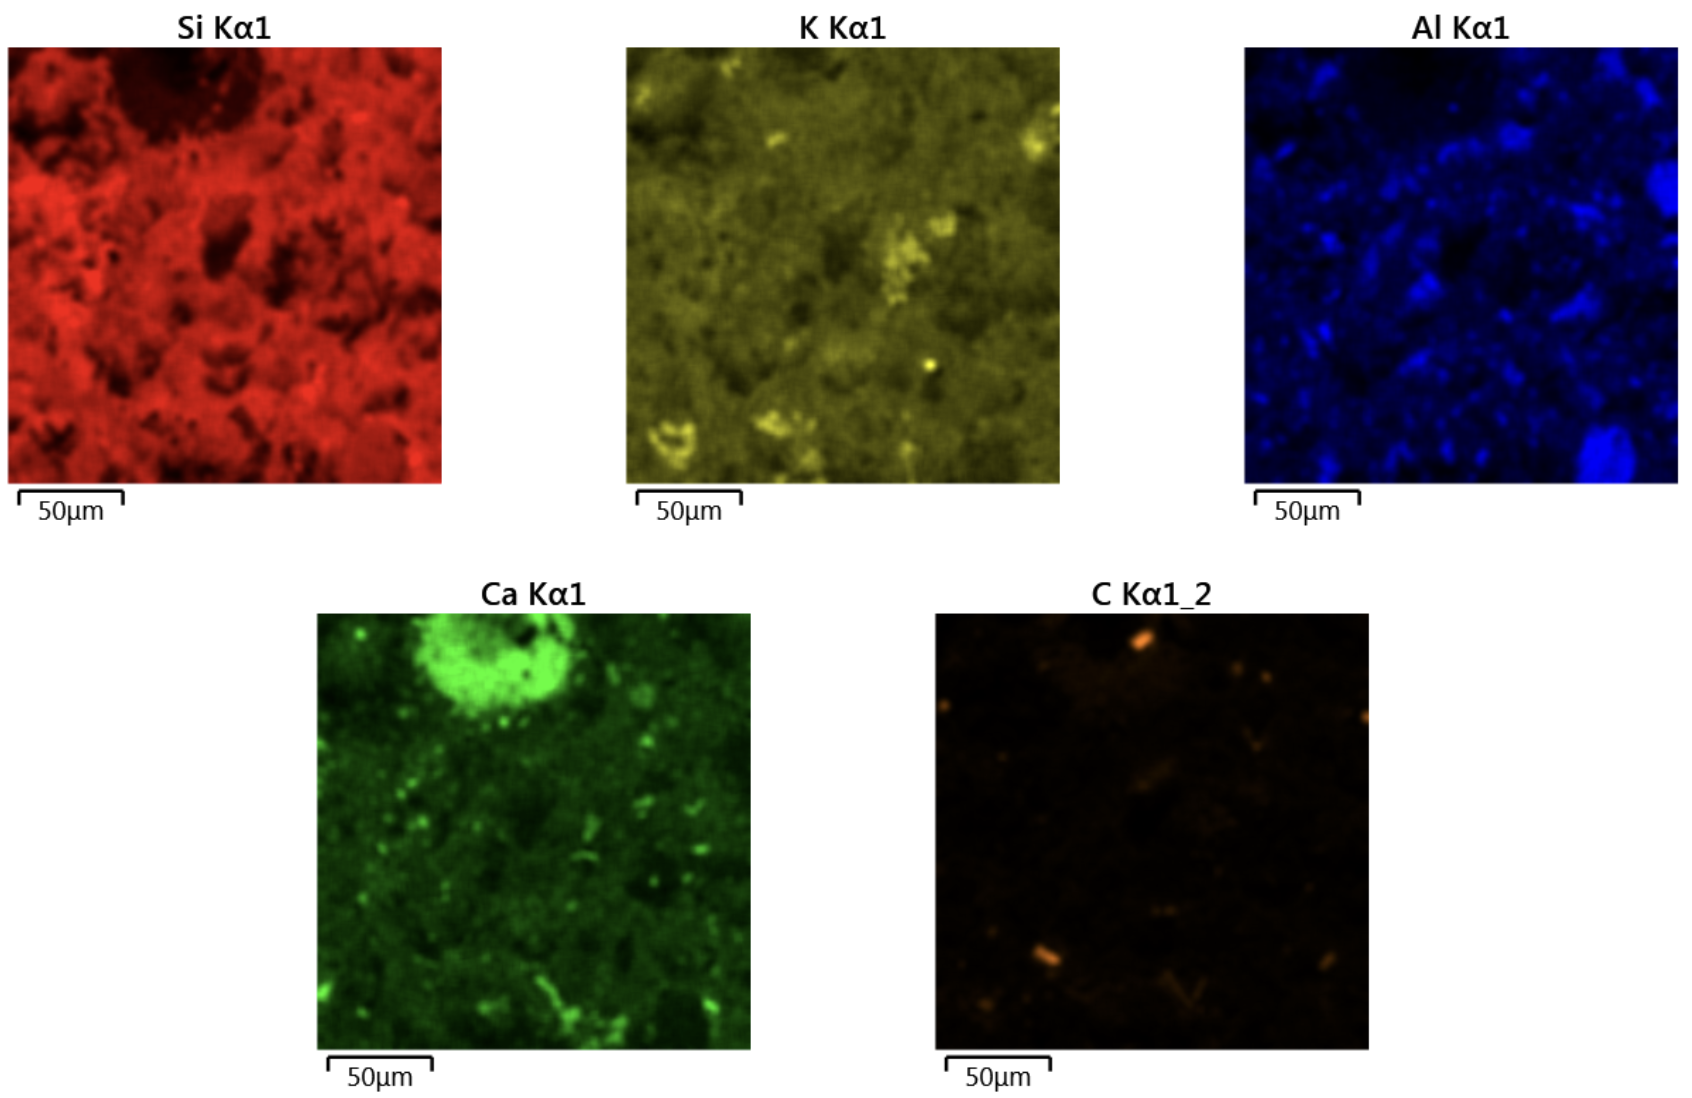
\includegraphics[height=6cm]{Cap4/images/5-0-60C-3d-Spot 1 - map.png}
    }
    \caption{EDS analysis of Spot 1, Si/Al = 5.0, cured for 3 days at 60°C at 1000× magnification.}
    \label{fig:eds_spot1_5-0}
\end{figure}

The spectrum results are summarized in Table \ref{tab:eds_spectrum} and it can be noted that the K/Ca ratio was approximately constant and equals to 2, as expected from the mix design.
However, the Si/Al ratio from EDS was slightly higher than the intended mix design values.
It can be speculated that this is due to a stronger tendency of Si to stays in solution rather than being incorporated into the gel structure and precipitate during geopolymerization at high pH environment \cite{chen2024synthesis}.
\textcolor{red}{Am I missing something?}

\begin{table}[H]
    \centering
    \caption{EDS spectrum of pastes after 3 days of curing at 60$\degree$C.}
    \label{tab:eds_spectrum}
    \begin{tabular}{c c c c c c c c c}
        \hline
        \multirow{2}{*}{Sample} & \multicolumn{4}{c}{At(\%)} & \multicolumn{4}{c}{Wt(\%)} \\
        \cline{2-9}
        & Si & Al & K & Ca & Si & Al & K & Ca \\
        \hline
        0.9\textunderscore 60C\textunderscore 3d\textunderscore Spot5 & 26.4 & 27.1 & 30.4 & 16.0 & 22.4 & 22.1 & 36.0 & 19.5 \\
        3.0\textunderscore 60C\textunderscore 3d\textunderscore Spot3 & 54.2 & 13.5 & 21.5 & 10.8 & 48.2 & 11.5 & 26.6 & 13.7 \\
        5.0\textunderscore 60C\textunderscore 3d\textunderscore Spot1 & 59.5 & 9.2 & 19.6 & 11.6 & 53.0 & 7.9 & 24.2 & 14.9 \\
        \hline
    \end{tabular}
\end{table}

Additional EDS spectral data for all analyzed spots can be found in Appendix \ref{appendix:eds_spectra}.

\section{Physical properties of Mortars}
\textcolor{red}{Which results we want from bulk density/ water absorption tests?}
\textcolor{red}{I think it would be better in a single table, but it may need to be on landscape}

\begin{landscape}
  \begin{table}[H]
    \centering
    \caption{Bulk density, water absorption, and permeable voids volume of mortars (curing for 3 days at 60$\degree$C).}
    \label{tab:bulk_density_water_absorption}
    \begin{tabular}{cccccccc}
      \hline
      % \multirow{2}{*}{Sample}        & Absorption (\%) & Mean $\pm$ deviation (\%) & Bulk density (g/cm$^3$) & Mean $\pm$ deviation (\%) & Permeable voids volume (\%) & Mean $\pm$ deviation (\%) \\
      \multirow{2}{*}{Sample}        & Absorption & Mean $\pm$  & Bulk density & Mean $\pm$ & Permeable voids  & Mean $\pm$\\
       & (\%) & deviation (\%) & (g/cm$^3$) & deviation (g/cm$^3$) & volume (\%) & deviation (\%) \\
      \hline
      0.9\_3d-60C-1 & 10.9 & \multirow{3}{*}{11.0 $\pm$ 0.1} & 2.405 & \multirow{3}{*}{2.407 $\pm$ 0.008} & 21.3 & \multirow{3}{*}{21.5 $\pm$ 0.2} \\
      0.9\_3d-60C-2 & 11.1 & & 2.401 & & 21.5 & \\
      0.9\_3d-60C-3 & 11.1 & & 2.416 & & 21.7 & \\
      2.0\_3d-60C-1 & 11.6 & \multirow{3}{*}{11.6 $\pm$ 0.1} & 2.392 & \multirow{3}{*}{2.401 $\pm$ 0.014} & 21.8 & \multirow{3}{*}{22.3 $\pm$ 0.7} \\
      2.0\_3d-60C-2 & 11.5 & & 2.393 & & 21.9 & \\
      2.0\_3d-60C-3 & 11.7 & & 2.417 & & 23.1 & \\
      3.0\_3d-60C-1 & 12.0 & \multirow{3}{*}{11.9 $\pm$ 0.1} & 2.415 & \multirow{3}{*}{2.425 $\pm$ 0.009} & 23.0 & \multirow{3}{*}{23.1 $\pm$ 0.3} \\
      3.0\_3d-60C-2 & 12.0 & & 2.428 & & 23.4 & \\
      3.0\_3d-60C-3 & 11.8 & & 2.433 & & 22.8 & \\
      4.0\_3d-60C-1 & 11.3 & \multirow{3}{*}{11.5 $\pm$ 0.2} & 2.403 & \multirow{3}{*}{2.404 $\pm$ 0.011} & 22.2 & \multirow{3}{*}{22.4 $\pm$ 0.2} \\
      4.0\_3d-60C-2 & 11.5 & & 2.416 & & 22.7 & \\
      4.0\_3d-60C-3 & 11.8 & & 2.393 & & 22.4 & \\
      5.0\_3d-60C-1 & 11.2 & \multirow{3}{*}{11.3 $\pm$ 0.3} & 2.393 & \multirow{3}{*}{2.399 $\pm$ 0.008} & 21.2 & \multirow{3}{*}{21.5 $\pm$ 0.4} \\
      5.0\_3d-60C-2 & 11.2 & & 2.396 & & 21.2 & \\
      5.0\_3d-60C-3 & 11.6 & & 2.409 & & 22.0 & \\
      \hline
    \end{tabular}
  \end{table}
\end{landscape}

% \begin{table}[H]
% \centering
% \caption{Compressive strength of mortars (curing for 1 day at 60$\degree$ C).}
% \label{tab:compressive_strength_1d}
% \begin{tabular}{cccc}
% \hline
% Si/Al Ratio & Sample & Compressive Strength (MPa) & Mean $\pm$ Std Dev (MPa) \\
% \hline
% \multirow{3}{*}{0.9} & 0.9\_1d-60C\_03 & 5.83 & \multirow{3}{*}{5.91 $\pm$ 0.08} \\
%  & 0.9\_1d-60C\_02 & 5.99 &  \\
%  & 0.9\_1d-60C\_01 & 5.92 &  \\
% \multirow{3}{*}{2.0} & 2.0\_1d-60C\_03 & 14.96 & \multirow{3}{*}{14.56 $\pm$ 0.64} \\
%  & 2.0\_1d-60C\_02 & 14.89 &  \\
%  & 2.0\_1d-60C\_01 & 13.82 &  \\
% \multirow{3}{*}{3.0} & 3.0\_1d-60C\_03 & 21.84 & \multirow{3}{*}{22.16 $\pm$ 0.82} \\
%  & 3.0\_1d-60C\_02 & 23.09 &  \\
%  & 3.0\_1d-60C\_01 & 21.55 &  \\
% \multirow{3}{*}{4.0} & 4.0\_1d-60C\_01 & 14.56 & \multirow{3}{*}{14.83 $\pm$ 0.25} \\
%  & 4.0\_1d-60C\_02 & 14.85 &  \\
%  & 4.0\_1d-60C\_03 & 15.06 &  \\
% \multirow{3}{*}{5.0} & 5.0\_1d-60C\_01 & 12.71 & \multirow{3}{*}{12.91 $\pm$ 0.21} \\
%  & 5.0\_1d-60C\_02 & 12.88 &  \\
%  & 5.0\_1d-60C\_03 & 13.14 &  \\
% \hline
% \end{tabular}
% \end{table}

% \begin{table}[H]
%   \centering
%   \caption{Compressive strength of mortars (curing for 3 day at 60$\degree$ C).}
%   \label{tab:compressive_strength_3d}
%   \begin{tabular}{cccc}
%     \hline
%     Si/Al Ratio & Sample & Compressive Strength (MPa) & Mean $\pm$ Std Dev (MPa) \\
%     \hline
%     \multirow{3}{*}{0.9} & 0.9\_3d-60C\_03 & 7.86 & \multirow{3}{*}{7.83 $\pm$ 0.40} \\
%     & 0.9\_3d-60C\_02 & 8.20 &  \\
%     & 0.9\_3d-60C\_01 & 7.41 &  \\
%     \multirow{3}{*}{2.0} & 2.0\_3d-60C\_03 & 13.88 & \multirow{3}{*}{14.44 $\pm$ 0.49} \\
%     & 2.0\_3d-60C\_02 & 14.66 &  \\
%     & 2.0\_3d-60C\_01 & 14.79 &  \\
%     \multirow{3}{*}{3.0} & 3.0\_3d-60C\_03 & 23.82 & \multirow{3}{*}{23.88 $\pm$ 0.35} \\
%     & 3.0\_3d-60C\_02 & 24.25 &  \\
%     & 3.0\_3d-60C\_01 & 23.55 &  \\
%     \multirow{3}{*}{4.0} & 4.0\_3d-60C\_01 & 14.61 & \multirow{3}{*}{16.85 $\pm$ 1.95} \\
%     & 4.0\_3d-60C\_02 & 18.19 &  \\
%     & 4.0\_3d-60C\_03 & 17.74 &  \\
%     \multirow{3}{*}{5.0} & 5.0\_3d-60C\_01 & 14.76 & \multirow{3}{*}{14.68 $\pm$ 0.08} \\
%     & 5.0\_3d-60C\_02 & 14.66 &  \\
%     & 5.0\_3d-60C\_03 & 14.61 &  \\
%     \hline
%   \end{tabular}
% \end{table}

\begin{table}[H]
\centering
\caption{Compressive strength of mortars cured at 60$\degree$C after 1 and 3 days.}
\label{tab:compressive_strength_combined}
\begin{tabular}{ccccc}
\hline
\multirow{2}{*}{Sample} &
\multicolumn{2}{c}{Compressive Strength (MPa)} &
\multicolumn{2}{c}{Mean $\pm$ Std Dev (MPa)} \\
\cline{2-5}
 & 1 day & 3 days & 1 day & 3 days \\
\hline
0.9-1 & 5.83 & 7.86 & \multirow{3}{*}{5.91 $\pm$ 0.08} & \multirow{3}{*}{7.83 $\pm$ 0.40} \\
0.9-2 & 5.99 & 8.20 & & \\
0.9-3 & 5.92 & 7.41 & & \\
2.0-1 & 14.96 & 13.88 & \multirow{3}{*}{14.56 $\pm$ 0.64} & \multirow{3}{*}{14.44 $\pm$ 0.49} \\
2.0-2 & 14.89 & 14.66 & & \\
2.0-3 & 13.82 & 14.79 & & \\
3.0-1 & 21.84 & 23.82 & \multirow{3}{*}{22.16 $\pm$ 0.82} & \multirow{3}{*}{23.88 $\pm$ 0.35} \\
3.0-2 & 23.09 & 24.25 & & \\
3.0-3 & 21.55 & 23.55 & & \\
4.0-1 & 14.56 & 14.61 & \multirow{3}{*}{14.83 $\pm$ 0.25} & \multirow{3}{*}{16.85 $\pm$ 1.95} \\
4.0-2 & 14.85 & 18.19 & & \\
4.0-3 & 15.06 & 17.74 & & \\
5.0-1 & 12.71 & 14.76 & \multirow{3}{*}{12.91 $\pm$ 0.21} & \multirow{3}{*}{14.68 $\pm$ 0.08} \\
5.0-2 & 12.88 & 14.66 & & \\
5.0-3 & 13.14 & 14.61 & & \\
\hline
\end{tabular}
\end{table}

\begin{figure}[H]
  \centering
  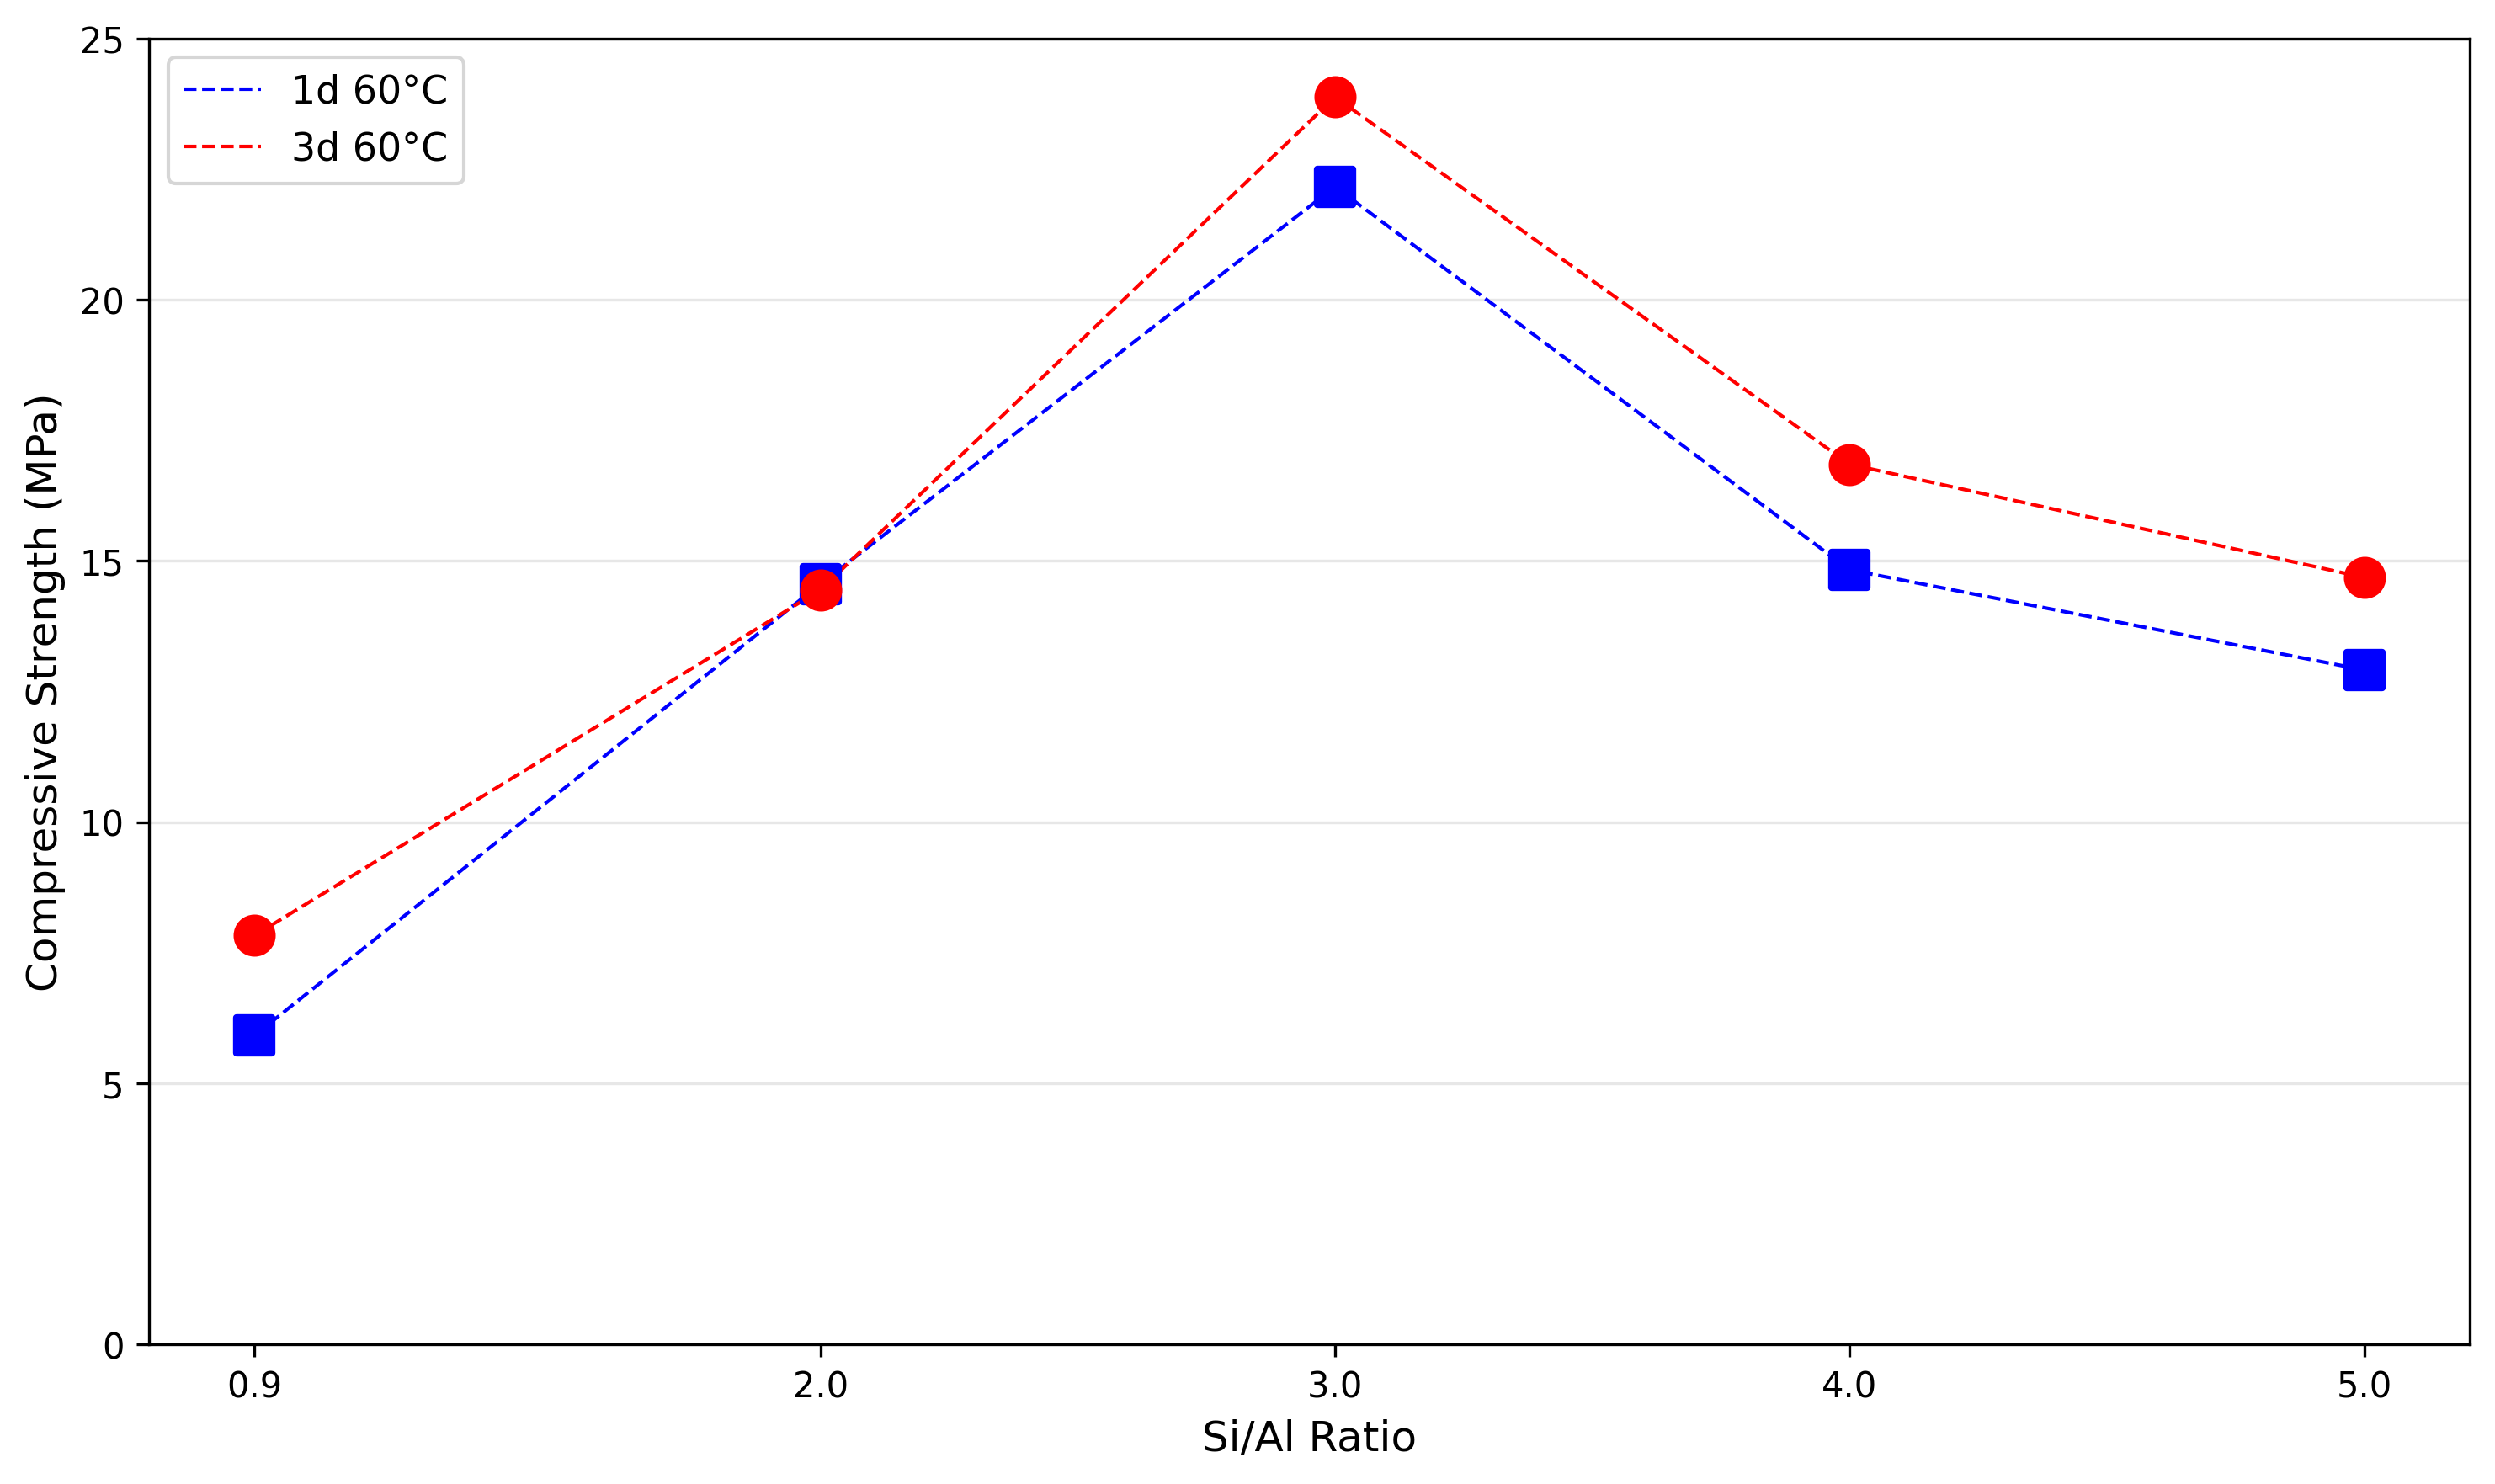
\includegraphics[width=0.75\textwidth]{Cap4/images/compression_strength_comparison_1d_vs_3d.png}
  \caption{Comparison of compressive strength for mortars cured for 1 day and 3 days at 60$\degree$C.}
  \label{fig:comparison_compression_strength}
\end{figure}